\documentclass[]{book}
\usepackage{lmodern}
\usepackage{amssymb,amsmath}
\usepackage{ifxetex,ifluatex}
\usepackage{fixltx2e} % provides \textsubscript
\ifnum 0\ifxetex 1\fi\ifluatex 1\fi=0 % if pdftex
  \usepackage[T1]{fontenc}
  \usepackage[utf8]{inputenc}
\else % if luatex or xelatex
  \ifxetex
    \usepackage{mathspec}
  \else
    \usepackage{fontspec}
  \fi
  \defaultfontfeatures{Ligatures=TeX,Scale=MatchLowercase}
\fi
% use upquote if available, for straight quotes in verbatim environments
\IfFileExists{upquote.sty}{\usepackage{upquote}}{}
% use microtype if available
\IfFileExists{microtype.sty}{%
\usepackage{microtype}
\UseMicrotypeSet[protrusion]{basicmath} % disable protrusion for tt fonts
}{}
\usepackage[margin=1in]{geometry}
\usepackage{hyperref}
\hypersetup{unicode=true,
            pdftitle={State Space Models in Stan},
            pdfauthor={Jeffrey B. Arnold},
            pdfborder={0 0 0},
            breaklinks=true}
\urlstyle{same}  % don't use monospace font for urls
\usepackage{biblatex}

\addbibresource{packages.bib}
\addbibresource{ssmodels-in-stan.bib}
\usepackage{color}
\usepackage{fancyvrb}
\newcommand{\VerbBar}{|}
\newcommand{\VERB}{\Verb[commandchars=\\\{\}]}
\DefineVerbatimEnvironment{Highlighting}{Verbatim}{commandchars=\\\{\}}
% Add ',fontsize=\small' for more characters per line
\usepackage{framed}
\definecolor{shadecolor}{RGB}{248,248,248}
\newenvironment{Shaded}{\begin{snugshade}}{\end{snugshade}}
\newcommand{\KeywordTok}[1]{\textcolor[rgb]{0.13,0.29,0.53}{\textbf{{#1}}}}
\newcommand{\DataTypeTok}[1]{\textcolor[rgb]{0.13,0.29,0.53}{{#1}}}
\newcommand{\DecValTok}[1]{\textcolor[rgb]{0.00,0.00,0.81}{{#1}}}
\newcommand{\BaseNTok}[1]{\textcolor[rgb]{0.00,0.00,0.81}{{#1}}}
\newcommand{\FloatTok}[1]{\textcolor[rgb]{0.00,0.00,0.81}{{#1}}}
\newcommand{\ConstantTok}[1]{\textcolor[rgb]{0.00,0.00,0.00}{{#1}}}
\newcommand{\CharTok}[1]{\textcolor[rgb]{0.31,0.60,0.02}{{#1}}}
\newcommand{\SpecialCharTok}[1]{\textcolor[rgb]{0.00,0.00,0.00}{{#1}}}
\newcommand{\StringTok}[1]{\textcolor[rgb]{0.31,0.60,0.02}{{#1}}}
\newcommand{\VerbatimStringTok}[1]{\textcolor[rgb]{0.31,0.60,0.02}{{#1}}}
\newcommand{\SpecialStringTok}[1]{\textcolor[rgb]{0.31,0.60,0.02}{{#1}}}
\newcommand{\ImportTok}[1]{{#1}}
\newcommand{\CommentTok}[1]{\textcolor[rgb]{0.56,0.35,0.01}{\textit{{#1}}}}
\newcommand{\DocumentationTok}[1]{\textcolor[rgb]{0.56,0.35,0.01}{\textbf{\textit{{#1}}}}}
\newcommand{\AnnotationTok}[1]{\textcolor[rgb]{0.56,0.35,0.01}{\textbf{\textit{{#1}}}}}
\newcommand{\CommentVarTok}[1]{\textcolor[rgb]{0.56,0.35,0.01}{\textbf{\textit{{#1}}}}}
\newcommand{\OtherTok}[1]{\textcolor[rgb]{0.56,0.35,0.01}{{#1}}}
\newcommand{\FunctionTok}[1]{\textcolor[rgb]{0.00,0.00,0.00}{{#1}}}
\newcommand{\VariableTok}[1]{\textcolor[rgb]{0.00,0.00,0.00}{{#1}}}
\newcommand{\ControlFlowTok}[1]{\textcolor[rgb]{0.13,0.29,0.53}{\textbf{{#1}}}}
\newcommand{\OperatorTok}[1]{\textcolor[rgb]{0.81,0.36,0.00}{\textbf{{#1}}}}
\newcommand{\BuiltInTok}[1]{{#1}}
\newcommand{\ExtensionTok}[1]{{#1}}
\newcommand{\PreprocessorTok}[1]{\textcolor[rgb]{0.56,0.35,0.01}{\textit{{#1}}}}
\newcommand{\AttributeTok}[1]{\textcolor[rgb]{0.77,0.63,0.00}{{#1}}}
\newcommand{\RegionMarkerTok}[1]{{#1}}
\newcommand{\InformationTok}[1]{\textcolor[rgb]{0.56,0.35,0.01}{\textbf{\textit{{#1}}}}}
\newcommand{\WarningTok}[1]{\textcolor[rgb]{0.56,0.35,0.01}{\textbf{\textit{{#1}}}}}
\newcommand{\AlertTok}[1]{\textcolor[rgb]{0.94,0.16,0.16}{{#1}}}
\newcommand{\ErrorTok}[1]{\textcolor[rgb]{0.64,0.00,0.00}{\textbf{{#1}}}}
\newcommand{\NormalTok}[1]{{#1}}
\usepackage{longtable,booktabs}
\usepackage{graphicx,grffile}
\makeatletter
\def\maxwidth{\ifdim\Gin@nat@width>\linewidth\linewidth\else\Gin@nat@width\fi}
\def\maxheight{\ifdim\Gin@nat@height>\textheight\textheight\else\Gin@nat@height\fi}
\makeatother
% Scale images if necessary, so that they will not overflow the page
% margins by default, and it is still possible to overwrite the defaults
% using explicit options in \includegraphics[width, height, ...]{}
\setkeys{Gin}{width=\maxwidth,height=\maxheight,keepaspectratio}
\IfFileExists{parskip.sty}{%
\usepackage{parskip}
}{% else
\setlength{\parindent}{0pt}
\setlength{\parskip}{6pt plus 2pt minus 1pt}
}
\setlength{\emergencystretch}{3em}  % prevent overfull lines
\providecommand{\tightlist}{%
  \setlength{\itemsep}{0pt}\setlength{\parskip}{0pt}}
\setcounter{secnumdepth}{5}
% Redefines (sub)paragraphs to behave more like sections
\ifx\paragraph\undefined\else
\let\oldparagraph\paragraph
\renewcommand{\paragraph}[1]{\oldparagraph{#1}\mbox{}}
\fi
\ifx\subparagraph\undefined\else
\let\oldsubparagraph\subparagraph
\renewcommand{\subparagraph}[1]{\oldsubparagraph{#1}\mbox{}}
\fi

%%% Use protect on footnotes to avoid problems with footnotes in titles
\let\rmarkdownfootnote\footnote%
\def\footnote{\protect\rmarkdownfootnote}

%%% Change title format to be more compact
\usepackage{titling}

% Create subtitle command for use in maketitle
\newcommand{\subtitle}[1]{
  \posttitle{
    \begin{center}\large#1\end{center}
    }
}

\setlength{\droptitle}{-2em}
  \title{State Space Models in Stan}
  \pretitle{\vspace{\droptitle}\centering\huge}
  \posttitle{\par}
  \author{Jeffrey B. Arnold}
  \preauthor{\centering\large\emph}
  \postauthor{\par}
  \predate{\centering\large\emph}
  \postdate{\par}
  \date{2016-12-01}

\usepackage{booktabs}

\DeclareMathOperator{\E}{E}
\DeclareMathOperator{\mean}{mean}
\DeclareMathOperator{\Var}{Var}
\DeclareMathOperator{\Cov}{Cov}
\DeclareMathOperator{\Cor}{Cor}
\DeclareMathOperator{\Bias}{Bias}
\DeclareMathOperator{\MSE}{MSE}
\DeclareMathOperator{\sd}{sd}
\DeclareMathOperator{\se}{se}
\DeclareMathOperator{\rank}{rank}
\DeclareMathOperator*{\argmin}{arg\,min}
\DeclareMathOperator*{\argmax}{arg\,max}
\DeclareMathOperator{\diag}{diag}
\DeclareMathOperator{\VEC}{vec}

\newcommand{\mat}[1]{\boldsymbol{#1}}
\renewcommand{\vec}[1]{\boldsymbol{#1}}
\renewcommand{\T}{'}

\newcommand{\distr}[1]{\mathcal{#1}}
\newcommand{\dnorm}{\distr{N}}
\newcommand{\dmvnorm}[1]{\distr{N}_{#1}}
\newcommand{\dt}[1]{\distr{T}_{#1}}

\newcommand{\cia}{\perp\!\!\!\perp}
\DeclareMathOperator*{\plim}{plim}

\begin{document}
\maketitle

{
\setcounter{tocdepth}{1}
\tableofcontents
}
\chapter{Introduction}\label{introduction}

This contains documentation for ``State Space Models in Stan''

\chapter{The Linear State Space
Model}\label{the-linear-state-space-model}

\autocite[Sec 3.1]{DurbinKoopman2012}

The linear Gaussian state space model (SSM)\footnote{This is also called
  a dynamic linear model (DLM).} the the \(n\)-dimensional observation
sequence \(\vec{y}_1, \dots, \vec{y}_n\), \[
\begin{aligned}[t]
\vec{y}_t &= \vec{d}_t + \mat{Z}_t \vec{\alpha}_t + \vec{\varepsilon}_t,  &
\vec{\varepsilon}_t & \sim N(0, \mat{H}_t), \\
\vec{\alpha}_{t + 1} &= \vec{c}_t + \mat{T}_t \vec{\alpha}_t + \mat{R}_t \vec{\eta}_t,  &
\vec{\eta}_t & \sim N(0, \mat{Q}_t), \\
&& \vec{\alpha}_1 &\sim N(\vec{a}_1, \mat{P}_1) .
\end{aligned}
\] for \(t = 1, \dots, n\). The first equation is called the
\emph{observation} or \emph{measurement equation}. The second equation
is called the \emph{state}, \emph{transition}, or \emph{system
equation}. The vector \(\vec{y}_t\) is a \(p \times 1\) vector called
the \emph{observation vector}. The vector \(\alpha{\alpha}_t\) is a
\(m \times 1\) vector called the \emph{state vector}. The matrices are
vectors, \(\mat{Z}_t\),\(\mat{T}_t\), \(\mat{R}_t\), \(\mat{H}_t\),
\(\mat{Q}_t\), \(c_t\), and \(d_t\) are called the \emph{system
matrices}. The system matrices are considered fixed and known in the
filtering and smoothing equations below, but can be parameters
themselves. The \(p \times m\) matrix \(\mat{Z}_t\) links the
observation vector \(\vec{y}_t\) with the state vector
\(\vec{\alpha}_t\). The \(m \times m\) transition matrix \(\mat{T}_t\)
determines the evolution of the state vector, \(\vec{\alpha}_t\). The
\(q \times 1\) vector \(\vec{\eta}_t\) is called the \emph{state
disturbance vector}, and the \(p \times 1\) vector
\(\vec{\varepsilon}_t\) is called the \emph{observation disturbance
vector}. An assumption is that the state and observation disturbance
vectors are uncorrelated,
\(\Cov(\vec{\varepsilon}_t, \vec{\eta}_t) = 0\).

In a general state space model, the normality assumptions of the
densities of \(\vec{\varepsilon}\) and \(\vec{\eta}\) are dropped.

In many cases \(\mat{R}_t\) is the identity matrix. It is possible to
define \(\eta^*_t = \mat{R}_t \vec{\eta}_t\), and
\(\mat{Q}^* = \mat{R}_t \mat{Q}_t' \mat{R}'_t\). However, if
\(\mat{R}_t\) is \(m \times q\) and \(q < m\), and \(\mat{Q}_t\) is
nonsingular, then it is useful to work with the nonsingular
\(\vec{\eta}_t\) rather than a singular \(\vec{\eta}_t^*\).

The initial state vector \(\vec{\alpha}_1\) is assume to be generated
as, \[
\alpha_1 \sim N(\vec{a}_1, \mat{P}_1)
\] independently of the observation and state disturbances
\(\vec{\varepsilon}\) and \(\vec{\eta}\). The values of \(\vec{a}_1\)
and \(\mat{P}_1\) can be considered as given and known in most
stationary processes. When the process is nonstationary, the elements of
\(\vec{a}_1\) need to be treated as unknown and estimated. This is
called \emph{initialization}.

\begin{longtable}[]{@{}lll@{}}
\caption{Dimensions of matrices and vectors in the SSM}\tabularnewline
\toprule
matrix/vector & dimension & name\tabularnewline
\midrule
\endfirsthead
\toprule
matrix/vector & dimension & name\tabularnewline
\midrule
\endhead
\(\vec{y}_t\) & \(p \times 1\) & observation vector\tabularnewline
\(\vec{\alpha}_t\) & \(m \times 1\) & (unobserved) state
vector\tabularnewline
\(\vec{\varepsilon}_t\) & \(m \times 1\) & observation disturbance
(error)\tabularnewline
\(\vec{\eta}_t\) & \(q \times 1\) & state disturbance
(error)\tabularnewline
\(\vec{a}_1\) & \(m \times 1\) & initial state mean\tabularnewline
\(\vec{c}_t\) & \(m \times 1\) & state intercept\tabularnewline
\(\vec{d}_t\) & \(p \times 1\) & observation intercept\tabularnewline
\(\mat{Z}_t\) & \(p \times m\) & design matrix\tabularnewline
\(\mat{T}_t\) & \(m \times m\) & transition matrix\tabularnewline
\(\mat{H}_t\) & \(p \times p\) & observation covariance
matrix\tabularnewline
\(\mat{R}_t\) & \(m \times q\) & state covariance selection
matrix\tabularnewline
\(\mat{Q}_t\) & \(q \times q\) & state covariance matrix\tabularnewline
\(\mat{P}_1\) & \(m \times m\) & initial state covariance
matrix\tabularnewline
\bottomrule
\end{longtable}

\chapter{Filtering and Smoothing}\label{filtering-and-smoothing}

\section{Filtering}\label{filtering}

From \autocite[Sec 4.3]{DurbinKoopman2012}

Let \(\vec{a}_t = \E(\vec{\alpha}_t | y_{1, \dots, t - 1})\) be the
expected value
\(\vec{P}_t = \Var(\vec{\alpha}_t | y_{1, \dots, t - 1})\) be the
variance of the state in \(t + 1\) given data up to time \(t\). To
calculate \(\vec{\alpha}_{t + 1}\) and \(\mat{P}_{t + 1}\) given the
arrival of new data at time \(t\), \[
\begin{aligned}[t]
\vec{v}_t &= \vec{y}_t - \mat{Z}_t \vec{a}_t - \vec{d}_t, \\
\mat{F}_t &= \mat{Z}_t \mat{P}_t \mat{Z}_t\T + \mat{H}_t, \\
\mat{K}_t &= \mat{T}_t \mat{P}_t \mat{Z}_t\T \mat{F}_t^{-1} \\
\vec{a}_{t + 1} &= \mat{T}_t \vec{a}_t + \mat{K}_t \vec{v}_t + \vec{c}_t \\
\mat{P}_{t + 1} &= \mat{T}_t \mat{P}_t (\mat{T}_t - \mat{K}_t \mat{Z}_t)\T + \mat{R}_t \mat{Q}_t \mat{R}_t\T .
\end{aligned}
\] The vector \(\vec{v}_t\) are the \emph{one-step ahead forecast
errors\$, and the matrix \(\mat{K}_t\) is called the }Kalman gain*.

The filter can also be written to estimate the \emph{filtered states},
where \(\vec{a}_{t|t} = \E(\vec{\alpha}_t | y_{1, \dots, t})\) is the
expected value and
\(\vec{P}_{t|t} = \Var(\vec{\alpha}_t | y_{1, \dots, t})\) is the
variance of the state \(\vec{\alpha}_t\) given information up to
\emph{and including} \(\vec{y}_t\). The filter written this way is, \[
\begin{aligned}[t]
\vec{v}_t &= \vec{y}_t - \mat{Z}_t \vec{a}_t - \vec{d}_t, \\
\mat{F}_t &= \mat{Z}_t \mat{P}_t \mat{Z}_t\T + \mat{H}_t, \\
\vec{a}_{t|t} &= \vec{a}_t + \mat{P}_t \mat{Z}_t\T \mat{F}_t^{-1} v_t , \\
\mat{P}_{t|t} &= \mat{P}_t - \mat{P}_t \mat{Z}_t\T \mat{F}_t^{-1} \mat{Z}_t \mat{P}_t , \\
\vec{a}_{t + 1} &= \mat{T}_{t} \vec{a}_{t|t} + \vec{c}_t, \\
\mat{P}_{t + 1} & = \mat{T}_t \mat{P}_{t|t} \mat{T}_t\T + \mat{R}_t \mat{Q}_t \mat{R}_t\T .
\end{aligned}
\]

\begin{longtable}[]{@{}ll@{}}
\caption{Dimensions of matrices and vectors in the SSM}\tabularnewline
\toprule
matrix/vector & dimension\tabularnewline
\midrule
\endfirsthead
\toprule
matrix/vector & dimension\tabularnewline
\midrule
\endhead
\(\vec{v}_t\) & \(p \times 1\)\tabularnewline
\(\vec{a}_t\) & \(m \times 1\)\tabularnewline
\(\vec{a}_{t|t}\) & \(m \times 1\)\tabularnewline
\(\mat{F}_t\) & \(p \times p\)\tabularnewline
\(\mat{K}_t\) & \(m \times p\)\tabularnewline
\(\mat{P}_t\) & \(m \times m\)\tabularnewline
\(\mat{P}_{t|T}\) & \(m \times m\)\tabularnewline
\(\vec{x}_t\) & \(m \times 1\)\tabularnewline
\(\mat{L}_t\) & \(m \times m\)\tabularnewline
\bottomrule
\end{longtable}

See \autocite[Sec 4.3.4]{DurbinKoopman2012}: For a time-invariant state
space model, the Kalman recursion for \(\mat{P}_{t + 1}\) converges to a
constant matrix \(\bar{\mat{P}}\), \[
\bar{\mat{P}} = \mat{T} \bar{\mat{P}} \mat{T}\T - \mat{T} \bar{\mat{P}} \mat{Z}\T \bar{\mat{F}}^{-1} \mat{Z} \bar{\mat{P}} \mat{T}\T + \mat{R} \mat{Q} \mat{R}\T ,
\] where \(\bar{\mat{F}} = \mat{Z} \bar{\mat{P}} \mat{Z}\T + \mat{H}\).

See \autocite[Sec 4.3.5]{DurbinKoopman2012}: The \emph{state estimation
error} is, \[
\vec{x}_t = \vec{\alpha}_t - \vec{a}_t,
\] where \(\Var(\vec{x}_t) = \mat{P}_t\). The \(v_t\) are sometimes
called \emph{innovations}, since they are the part of \(\vec{y}_t\) not
predicted from the past. The innovation analog of the state space model
is \[
\begin{aligned}[t]
\vec{v}_t &= \mat{Z}_t \vec{x}_t + \vec{\varepsilon}_t ,  \\
\vec{x}_{t + 1} &= \mat{L} \vec{x}_{t} + \mat{R}_t \vec{\eta}_t - \mat{K}_t \vec{\varepsilon}_t , \\
\mat{K}_t &= \mat{T}_t \mat{P}_t \mat{Z}_t\T \mat{F}_t^{-1} , \\
\mat{L}_t &= \mat{T}_t - \mat{K}_t \mat{Z}_t ,
\mat{P}_{t + 1} &= \mat{T}_t \mat{P}_t \mat{L}_t\T +  \mat{R}_t \mat{Q}_t \mat{R}_T\T  .
\end{aligned}
\] These recursions allow for a simpler derivation of
\(\mat{P}_{t + 1}\), and are useful for the smoothing recursions.
Moreover, the one-step ahead forecast errors are indendendent, which
allows for a simple derivation of the log-likelihood.

Alternative methods \textbf{TODO}

\begin{itemize}
\tightlist
\item
  square-root filtering
\item
  precision filters
\item
  sequential filtering
\end{itemize}

\section{Smoothing}\label{smoothing}

While filtering calculates the conditional densities the states and
disturbances given data prior to or up to the current time, smoothing
calculates the conditional densities states and disturbances given the
entire series of observations, \(\vec{y}_{1:n}\).

\emph{State smoothing} calculates the conditional mean,
\(\hat{\vec{\alpha}}_t = \E(\vec{\alpha}_t | \vec{y}_{1:n})\), and
variance, \(\mat{V}_t = \Var(\vec{\alpha}_t | \vec{y}_{1:n})\), of the
states. Observation disturbance smoothing calculates the conditional
mean,
\(\hat{\vec{\varepsilon}}_t = \E(\vec{\varepsilon}_t | \vec{y}_{1:n})\),
and variance, \(\Var(\vec{\varepsilon}_t | \vec{y}_{1:n})\), of the
state disturbances. Likewise, state disturbance smoothing calculates the
conditional mean,
\(\hat{\vec{\eta}}_t = \E(\vec{\eta}_t | \vec{y}_{1:n})\), and variance,
\(\Var(\vec{\eta}_t | \vec{y}_{1:n})\), of the state disturbances.

\begin{longtable}[]{@{}ll@{}}
\caption{Dimensions of vectors and matrices used in smoothing
recursions}\tabularnewline
\toprule
Vector/Matrix & Dimension\tabularnewline
\midrule
\endfirsthead
\toprule
Vector/Matrix & Dimension\tabularnewline
\midrule
\endhead
\(\vec{r}_t\) & \(m \times 1\)\tabularnewline
\(\vec{\vec{\alpha}}_t\) & \(m \times 1\)\tabularnewline
\(\vec{u}_t\) & \(p \times 1\)\tabularnewline
\(\hat{\vec{\varepsilon}}_t\) & \(p \times 1\)\tabularnewline
\(\hat{\vec{\eta}}_t\) & \(r \times 1\)\tabularnewline
\(\mat{N}_t\) & \(m \times m\)\tabularnewline
\(\mat{V}_t\) & \(m \times m\)\tabularnewline
\(\mat{D}_t\) & \(p \times p\)\tabularnewline
\bottomrule
\end{longtable}

\subsection{State Smoothing}\label{state-smoothing}

Smoothing calculates conditional density of the states given all
observations, \(p(\vec{\alpha} | \vec{y}_{1:n})\). Let
\(\hat{\vec{\alpha}} = \E(\vec{\alpha}_t | \vec{y}_{1:n})\) be the mean
and \(\mat{V}_t = \Var(\vec{\alpha} | \vec{y}_{1:n})\) be the variance
of this density. The following recursions can be used to calculate these
densities \autocite[Sec 4.4.4]{DurbinKoopman2012}, \[
\begin{aligned}[t]
\vec{r}_{t - 1} &= \mat{Z}_t\T \mat{F}_t^{-1} \vec{v}_t + \mat{L}_t\T \vec{r}_t , &
\mat{N}_{t - 1} &= \mat{Z}_t\T \mat{F}_t^{-1} \mat{Z}_t + \mat{L}_t\T \mat{N}_t \mat{L}_t, \\
\hat{\vec{\alpha}}_t &= \vec{a}_t + \mat{P}_t \vec{r}_{t - 1} , &
\mat{V}_t &= \mat{P}_t - \mat{P}_t \mat{N}_{t - 1} \mat{P}_t ,
\end{aligned}
\] for \(t = n, \dots, 1\), with \(\vec{r}_n = \vec{0}\), and
\(\mat{N}_n = \mat{0}\).

During the filtering pass \(\vec{v}_t\), \(\mat{F}_t\), \(\mat{K}_t\),
and \(\mat{P}_t\) for \(t = 1, \dots, n\) need to be stored.
Alternatively, \(\vec{a}_t\) and \(\mat{P}_t\) only can be stored, and
\(\vec{v}_t\), \(\mat{F}_t\), \(\mat{K}_t\) recalculated on the fly.
However, since the dimensions of \(\vec{v}_t\), \(\mat{F}_t\),
\(\mat{K}_t\) are usually small relative to \(\vec{a}_t\) and
\(\mat{P}_t\) is is usually worth storing them.

\subsection{Disturbance smoothing}\label{disturbance-smoothing}

Disturbance smoothing calculates the density of the state and
observation disturbances (\(\vec{\eta}_t\) and \(\vec{\varepsilon}_t\))
given the full series of observations \(\vec{y}_{1:n}\). Let
\(\hat{\vec{\varepsilon}}_t = \E(\vec{\varepsilon} | \vec{y}_{1:n})\) be
the mean and \(\Var(\vec{\varepsilon}_t | \vec{y}_{1:n})\) be the
variance of the smoothed density of the observation disturbances at time
\(t\), \(p(\vec{\varepsilon}_t | \vec{y}_{1:n})\). Likewise, let
\(\hat{\vec{\eta}} = \E(\vec{\eta}_t | \vec{y}_{1:n})\) be the mean and
\(\Var(\vec{\eta}_t | \vec{y}_{1:n})\) be the variance of the smoothed
density of the state disturbances at time \(t\),
\(p(\vec{\eta}_t | \vec{y}_{1:n})\). The following recursions can be
used to calculate these values \autocite[Eq 4.69]{DurbinKoopman2012}: \[
\begin{aligned}[t]
\hat{\vec{\varepsilon}}_t &= \mat{H}_t (\mat{F}^{-1} \vec{v}_t - \mat{K}_t\T \vec{r}_t) , &
\Var(\vec{\varepsilon}_t | \mat{Y}_n) &= \mat{H}_t - \mat{H}_t (\mat{F}_t^{-1} + \mat{K}_t\T \mat{N}_t \mat{K}_t) \mat{H}_t , \\
\hat{\vec{\eta}}_t &= \mat{Q}_t \mat{R}_t\T \vec{r}_t , &
\Var(\vec{\eta}_t | \mat{Y}_n) &= \mat{Q}_t - \mat{Q}_t \mat{R}_t\T \mat{N}_t \mat{R}_t \mat{Q}_t , \\
\vec{r}_{t - 1} &= \mat{Z}_t\T \mat{F}_t^{-1} \vec{v}_t + \mat{L}_t\T \vec{r}_t , &
\mat{N}_{t - 1} &= \mat{Z}_t\T \mat{F}_t^{-1} \mat{Z}_t + \mat{L}_t\T \mat{N}_t \mat{L}_t
\end{aligned}
\] Alternatively, these equations can be rewritten as \autocite[Sec
4.5.3]{DurbinKoopman2012}: \[
\begin{aligned}[t]
\hat{\vec{\varepsilon}}_t &= \mat{H}_t \vec{u}_t , &
\Var(\vec{\varepsilon}_t | \mat{Y}_n) &= \mat{H}_t - \mat{H}_t \mat{D}_t \mat{H}_t , \\
\hat{\vec{\eta}}_t &= \mat{Q}_t \mat{R}_t\T \vec{r}_t , &
\Var(\vec{\eta}_t | \mat{Y}_n) &= \mat{Q}_t - \mat{Q}_t \mat{R}_t\T \mat{N}_t \mat{R}_t \mat{Q}_t , \\
\vec{u}_t &= \mat{F}^{-1} \vec{v}_t - \mat{K}_t\T \vec{r}_t , &
\mat{D}_t &= \mat{F}_t^{-1} + \mat{K}_t\T \mat{N}_t \mat{K}_t , \\
\vec{r}_{t - 1} &= \mat{Z}_t\T \vec{u}_t + \mat{T}_t\T \vec{r}_t , &
\mat{N}_{t - 1} &= \mat{Z}_t\T \mat{D}_t \mat{Z}_t + \mat{T}_t\T \mat{N}_t \mat{T}_t - \mat{Z}_t\T \mat{K}_t\T \mat{N}_t \mat{T}_t - \mat{T}_t\T \mat{N}_t \mat{K}_t \mat{Z}_t .
\end{aligned}
\] This reformulation can be computationally useful since it relies on
the system matrices \(\mat{Z}_t\) and \(\mat{T}_t\) which are often
sparse. The disturbance smoothing recursions require only \(\vec{v}_t\),
\(\mat{f}_t\), and \(\mat{K}_t\) which are calculated with a forward
pass of the Kalman filter. Unlike the state smoother, the disturbance
smoothers do not require either the mean (\(\vec{a}_t\)) or variance
(\(\mat{P}_t\)) of the predicted state density.

\subsection{Fast state smoothing}\label{fast-state-smoothing}

If the variances of the states do not need to be calculated, then a
faster smoothing algorithm can be used (Koopman 1993). The fast state
smoother is defined as \autocite[Sec 4.6.2]{DurbinKoopman2012}, \[
\begin{aligned}[t]
\hat{\vec{\alpha}}_t &= \mat{T}_t \hat{\vec{\alpha}}_t + \mat{R}_t \mat{Q}_t \mat{R}_t\T \vec{r}_t , && t = 2, \dots, n \\
\hat{\vec{\alpha}}_1 &= \vec{a}_1 + \mat{P}_1 \vec{r}_0 .
\end{aligned}
\] The values of \(\vec{r}_t\) come from the recursions in the
disturbance smoother.

\section{Simulation smoothers}\label{simulation-smoothers}

Simulation smoothing draws samples of the states,
\(p(\vec{\alpha}_1, \dots, \vec{\alpha}_n | \vec{y}_{1:n})\), or
disturbances,
\(p(\vec{\varepsilon}_1, \dots, \vec{\varepsilon}_n | \vec{y}_{1:n})\)
and
\(p(\vec{\eta}_1, \dots, \vec{\eta}_n | \vec{y}_{1:n})\).{[}\^{}simsmo{]}

\subsection{Mean correction simulation
smoother}\label{mean-correction-simulation-smoother}

The mean-correction simulation smoother was introduced in
\textcite{DurbinKoopman2002} . See \textcite{DurbinKoopman2012} (Sec
4.9) for an exposition of it. It requires only the previously described
filters and smoothers, and generating samples from multivariate
distributions.

\subsubsection{Disturbances}\label{disturbances}

\begin{enumerate}
\def\labelenumi{\arabic{enumi}.}
\tightlist
\item
  Run a filter and disturbance smoother to calculate
  \(\hat{\vec{\varepsilon}}_{1:n}\) and \(\hat{\vec{\eta}}_{1:(n - 1)}\)
\item
  Draw samples from the unconditional distribution of the disturbances,
  \[
  \begin{aligned}[t]
  \vec{\eta}^+_t &\sim N(0, \mat{H}_t) && t = 1, \dots, n - 1 \\
  \vec{\varepsilon}^+_t &\sim N(0, \mat{Q}_t) && t = 1, \dots, n
  \end{aligned}
  \]
\item
  Simulate observations from the system using the simulated
  disturbances, \[
  \begin{aligned}[t]
  \vec{y}^+_t &= \vec{d}_t + \mat{Z}_t \vec{\alpha}_t + \vec{\varepsilon}^+_t, \\
  \vec{\alpha}_{t + 1} &= \vec{c}_t + \mat{T}_t \vec{\alpha}_t + \mat{R}_t \vec{\eta}^+_t, \\
  \end{aligned}
  \] where \(\vec{\alpha}_1 \sim N(\vec{a}_1, \mat{P}_1)\).
\item
  Run a filter and disturbance smoother on the simulated observations
  \(\vec{y}^+\) to calculate
  \(\hat{\vec{\varepsilon}}_t^+ = \E(\vec{\varepsilon}_t | \vec{y}^+_{1:n})\)
  and \(\hat{\vec{\eta}}_t^+ = \E(\vec{\eta}_t | \vec{y}^+_{1:n})\).
\item
  A sample from
  \(p(\hat{\vec{\eta}}_{1:(n - 1)}, \hat{\vec{\varepsilon}}_{1:n} | \vec{y}_{1:n})\)
  is \[
  \begin{aligned}[t]
  \tilde{\vec{\eta}}_t &= \vec{\eta}^+_t - \hat{\vec{\eta}}^+_t + \hat{\vec{\eta}}_t , \\
  \tilde{\vec{\varepsilon}}_t &= \vec{\varepsilon}^+_t - \hat{\vec{\varepsilon}}^+_t + \hat{\vec{\varepsilon}}_t .
  \end{aligned}
  \]
\end{enumerate}

\subsubsection{States}\label{states}

\begin{enumerate}
\def\labelenumi{\arabic{enumi}.}
\tightlist
\item
  Run a filter and disturbance smoother to calculate the mean of the
  states conditional on the full series of observations,
  \(\hat{\vec{\alpha}}_{1:n} = \E(\vec{\alpha}_{1:n} | \vec{y}_{1:n})\).
\item
  Draw samples from the unconditional distribution of the disturbances,
  \[
  \begin{aligned}[t]
  \vec{\eta}^+_t &\sim N(0, \mat{H}_t) && t = 1, \dots, n - 1 \\
  \vec{\varepsilon}^+_t &\sim N(0, \mat{Q}_t) && t = 1, \dots, n
  \end{aligned}
  \]
\item
  Simulate states and observations from the system using the simulated
  disturbances, \[
  \begin{aligned}[t]
  \vec{y}^+_t &= \vec{d}_t + \mat{Z}_t \vec{\alpha}_t + \vec{\varepsilon}^+_t, \\
  \vec{\alpha}^+_{t + 1} &= \vec{c}_t + \mat{T}_t \vec{\alpha}_t + \mat{R}_t \vec{\eta}^+_t, \\
  \end{aligned}
  \] where \(\vec{\alpha}^+_1 \sim N(\vec{a}_1, \mat{P}_1)\).
\item
  Run a filter and smoother on the simulated observations \(\vec{y}^+\)
  to calculate
  \(\hat{\vec{\alpha}}_t^+ = \E(\vec{\alpha}_t | \vec{y}^+_{1:n})\).
\item
  A sample from \(p(\hat{\vec{\alpha}}_{1:n} | \vec{y}_{1:n})\) is \[
  \begin{aligned}[t]
  \tilde{\vec{\alpha}}_t &= \vec{\alpha}^+_t - \hat{\vec{\alpha}}^+_t + \hat{\vec{\alpha}}_t .
  \end{aligned}
  \]
\end{enumerate}

One convenient feature of this method is that since only the conditional
means of the states are required, the fast state smoother can be used,
since the variances of the states are not required.

\subsection{de Jong-Shephard method}\label{de-jong-shephard-method}

These recursions were developed in \textcite{DeJongShephard1995} .
Although the the mean-correction simulation smoother will work in most
cases, there are a few in which it will not work.

\textbf{TODO}

\subsection{Forward-filter backwards-smoother
(FFBS)}\label{forward-filter-backwards-smoother-ffbs}

This was the simulation method developed in \textcite{CarterKohn1994}
and \textcite{Fruehwirth-Schnatter1994} .

\textbf{TODO}

\section{Missing observations}\label{missing-observations}

When all observations at time \(t\) are missing, the filtering
recursions become \autocite[Sec 4.10]{DurbinKoopman2012}, \[
\begin{aligned}[t]
\vec{a}_{t|t} &= \vec{a}_t , \\
\mat{P}_{t|t} &= \mat{P}_t , \\
\vec{a}_{t + 1} &= \mat{T}_t \vec{a}_t + \vec{c}_t \\
\mat{P}_{t + 1} &= \mat{T}_t \mat{P}_t \mat{T}_t\T + \mat{R}_t \mat{Q}_t \mat{R}_t\T
\end{aligned}
\] This is equivalent to setting \(\mat{Z}_t = \mat{0}\) (implying also
that \(\mat{K}_t = \mat{0}\)) in the filtering equations. For smoothing,
also replace \(\mat{Z}_t = \mat{0}\), \[
\begin{aligned}[t]
\vec{r}_{t - 1} &= \mat{T}_t\T \vec{r}_t , \\
\mat{N}_{t - 1} &= \mat{T}_t\T \mat{N}_t \mat{T}_t,
\end{aligned}
\]

When some, but not all observations are missing, replace the observation
equation by, \[
\begin{aligned}[t]
\vec{y}^*_t &= \mat{Z}^*_t \vec{\alpha}_t + \vec{\varepsilon}_t^*, & \vec{\varepsilon}_t^* &\sim N(\vec{0}, \mat{H}_t^*),
\end{aligned}
\] where, \[
\begin{aligned}[t]
\vec{y}^*_t &= \mat{W}_t \vec{y}_t, \\
\mat{Z}^* &= \mat{W}_t \mat{Z}_t , \\
\vec{\varepsilon}_t &= \mat{W}_t \vec{\varepsilon}_t , \\
\mat{H}^*_t &= \mat{W}_t \mat{H}_t \mat{W}_t\T ,
\end{aligned}
\] and \(\mat{W}_t\) is a selection matrix to select non-missing values.
In smoothing the missing elements are estimated by the appropriate
elements of \(\mat{Z}_t \hat{\vec{alpha}}_t\), where
\(\hat{\vec{\alpha}}_t\) is the smoothed state.

\textbf{Note} If \(y_{t,j}\) is missing, then setting the relevant
entries in the forecast precision matrix, \(F^{-1}_{t,j,.} = \vec{0}\)
and \(F^{-1}_{t,.,j} = \vec{0}\), and Kalman gain matrix,
\(K_{t,.,j} = \vec{0}\), will handle missing values in the smoothers
without having to pass that information to the smoother. However, it may
be computationally more efficient if the values of the locations of the
missing observations are known.

\textbf{Note} For the disturbance and state simulation smoothers, I
think the missing observations need to be indicated and used when doing
the simulations on the state smoother.

\section{Forecasting matrices}\label{forecasting-matrices}

Forecasting future observations are the same as treating the future
observations as missing \autocite[Sec 4.11]{DurbinKoopman2012}, \[
\begin{aligned}[t]
\bar{\vec{y}}_{n + j} &= \mat{Z}_{n + j} \bar{\vec{a}}_{n + j} \\
\bar{\mat{F}}_{n + j} &= \mat{Z}_{n + j} \bar{\mat{P}}_{n + j} \mat{Z}_{n + j}\T + \mat{H}_{n + j} .
\end{aligned}
\]

\section{Univariate Representation of Multivariate
Series}\label{univariate-representation-of-multivariate-series}

See \autocite[Ch 6]{DurbinKoopman2012}

If \(\mat{H}_t\) is diagonal, then the vector series can be treated as a
univariate series for filtering and smoothing. This simplifies and has
computational benefits over the classic filtering and smoothing
algorithm because it avoids inverting \(\mat{F}_t\). Let, \[
\begin{aligned}[t]
\vec{y}_t &= \mat{Z} \vec{\alpha}_t + \vec{\varepsilon} & \vec{\varepsilon}_t &\sim N(\vec{0}, \mat{H}_t) \\
\vec{alpha}_{t + 1} &= \mat{T}_t \vec{\alpha}_t + \mat{R}_t \vec{\eta}_t & \vec{\eta}_t & \sim N(\vec{0}, \mat{Q}_t) \\
\alpha_1 & \sim N(\vec{a}_1, \mat{P}_1)
\end{aligned}
\] where \(\mat{H}_t\) is diagonal. The dimensions observation vector
are allowed to vary over time, with \(p_t\) being the size of the
observation vector at time \(t\). In this formulation, \(y_{t,i}\),
\(\varepsilon_{t,i}\) and \(\sigma^2_{t,i}\) are scalars, and
\(\vec{Z}_{t,i}\) is a length \(p_t\) row vector.

The observation equation in the univariate representation is \[
\begin{aligned}[t]
y_{t, i} = d_{t, i} + \vec{Z}_{t, i} \vec{\alpha}_t + \varepsilon_{t, i},  i = 1, \dots, p_t,  t = 1, \dots, n ,
\end{aligned}
\] and the state equation is, \[
\begin{aligned}[t]
\alpha_{t, i + 1} &= \alpha_t, & i &= 1, \dots, p_{t} - 1, \\
\alpha_{t + 1, 1} &= \vec{c}_t + \mat{T}_t \alpha_t, & t &= 1, \dots, n
\end{aligned}
\]

\subsection{Filtering}\label{filtering-1}

Define the following, \[
\begin{aligned}[t]
a_{t,1} &= \E(\alpha_{t,1} | \vec{y}_{1:t-1}) \\
P_{t,1} &= \Var(\alpha_{t,1} | \vec{y}_{1:t-1}) \\
a_{t,i} &= \E(\alpha_{t,1} | \vec{y}_{1:t-1}, y_{t,1}, \dots, y_{t,i - 1} \\
P_{t,i} &= \Var(\alpha_{t,1} | \vec{y}_{1:t-1}, y_{t,1}, \dots, y_{t,i - 1} \\  
\end{aligned}
\]

Given the univariate series, \[
y_{1,1}, \dots, y_{1,p_1}, y_{2,1}, \dots, y_{n - 1, p_{n -1}}, y_{n,1}, \dots, y_{n, p_n} .
\] The filtering steps as each \(y_{t,i}\) is processed is \[
\begin{aligned}[t]
v_{t,i} &= y_{t,i} - \vec{Z}_{t,i} \vec{a}_{t,i} - d_{t,i}, \\
F_{t,i} &= \vec{Z}_{t,i} \mat{P}_{t,i} \vec{Z}_{t,i}\T + \sigma^2_{t,i}, \\
\vec{K}_{t, i} &= \mat{P}_{t,i} \vec{Z}_{t,i}\T F^{-1}_{t,i}, \\
\vec{a}_{t, i + 1} &= \vec{a}_{t,i} + \vec{K}_{t,i} v_{t,i}, \\
\mat{P}_{t, i + 1} &= \mat{P}_{t,i} - \vec{K}_{t,i} F_{t,i} \vec{K}_{t,i}\T ,
\end{aligned}
\] for \(i = 1, \dots, p_t\). The prediction step to transition from
time \(t\) to \(t + 1\) is \[
\begin{aligned}[t]
\vec{a}_{t + 1, 1} &= \mat{T}_t \vec{a}_{t, p_t + 1} \\
\mat{P}_{t + 1, 1} &= \mat{T}_t \mat{P}_{t,p_t + 1} \mat{T}_t\T + \mat{R}_t \mat{Q}_t \mat{R}_t \T .
\end{aligned}
\] The values of \(\vec{a}_{t + 1, 1}\) and \(\mat{P}_{t + 1, 1}\) are
the same as the values of \(\vec{a}_{t + 1}\) and \(\mat{P}_{t + 1}\) in
the standard Kalman filter. Note that the values of \(v_{t,i}\),
\(\vec{K}_{t,i}\), and \(F_{t,i}^{-1}\) are not the same.

The SsfPack funtion \texttt{KalmanFilEx} stores (Doorback, p.~111) for
\((m + 2) \times n p\), \[
\begin{bmatrix}
v_{1,1} \dots v_{1,p} & \dots & v_{n, 1} \dots v_{n, p} \\
K_{1,1} \dots K_{1,p} & \dots & K_{n, p} \dots K_{n, p} \\
F^{-1}_{1,1} \dots F^{-1}_{1,p} & \dots & F^{-1}_{n,1} \dots F^{-1}_{n,p}
\end{bmatrix}
\]

\subsection{Smoothing}\label{smoothing-1}

The smoothing recursions for the univariate series \[
y_{1,1}, \dots, y_{1,p}, y_{2,1}, \dots, y_{n,p},
\] as \[
\begin{aligned}[t]
\vec{r}_{t,i - 1} &=
\mat{Z}_{t,i}\T F^{-1}_{t,i} v_{t,i} + \mat{L}_{t,i}\T \vec{r}_{t,i} &
\mat{N}_{t,i - 1} &= \mat{Z}_{t,i}\T F_{t,i}^{-1} \mat{Z}_{t,i} + \mat{L}_{t,i}\T \mat{N}_{t,i} \mat{L}_{t,i} ,
\vec{r}_{t - 1,p} &=
\mat{T}_{t - 1}\T \vec{r}_{t,0} &
\mat{N}_{t - 1, p} &= \mat{T}_{t-1}\T \mat{N}_{t,0} \mat{T}_{t - 1} ,
\end{aligned}
\] where \(\mat{L}_{t,i} = \mat{I}_{m} - \mat{K}_{t,i} \mat{Z}_{t,i}\),
for \(i = p, \dots, 1\) and \(t = n, \dots, 1\). The smoothing
recursions are initialized with \(\vec{r}_{n, p} = \vec{0}\) and
\(\mat{N}_{n,p} = \mat{0}\). The recursions for \(\vec{r}_{t-1, p}\) and
\(\mat{N}_{t - 1, p}\) are not used for \(t = 1\). The values of
\(\vec{r}_{t,0}\) and \(\mat{N}_{t,0}\) are equivalent to the values of
\(\vec{r}_{t-1}\) and \(\mat{N}_{t-1}\) in the standard smoothing
recursions.

The smoothed state vector
\(\hat{\vec{\alpha}}_t = \E(\vec{\alpha}_t | \vec{y}_{1:n})\) and
\(\mat{V}_t = \Var(\vec{\alpha}_t | \vec{y}_{1:n})\) are calculated
using the standard smoothing recursions with \[
\vec{a}_t &= \vec{a}_{t,1}, &
\mat{P}_t &= \mat{P}_{t,1}, &
\vec{r}_{t-1} &= \vec{r}_{t,0}, &
\mat{N}_{t-1} &= \mat{N}_{t,0}  .
\]

For the smoothed observation disturbances are calculated with, \[
\begin{aligned}[t]
\hat{\varepsilon}_{t,i} &= \sigma^2_{t,i} F^{-1}_{t,i} (v_{t,i} - \mat{K}_{t,i}\T \vec{r}_{t,i}) , \\
\Var(\hat{\varepsilon}_{t,i}) &= \sigma^4_{t,i} F^{-2}_{t,i} (F_{t,i} + \mat{K}_{t,i}\T \mat{N}_{t,i} \mat{K}_{t,i}) .
\end{aligned}
\]

The time reversion equation is, \[
\begin{aligned}[t]
\vec{r,p} &= \mat{T}_{t}\T \vec_{t + 1, 0} & \mat{N}_{t,p} = \mat{T}_t\T \mat{N}_{t + 1,0} \mat{T}_t,
\end{aligned}
\] for \(t = n, \dots, 1\). The recursion is initialized with
\(\vec{r}_{n + 1,0} = \vec{0}\) and \(\mat{N}_{n + 1, 0} = \mat{0}\).

The smoothing goes backwards through \(y_{t, p}, \dots, y_{t, 1}\), \[
\begin{aligned}[t]
& & \mat{K}_{t,i} &= \mat{N}_{t,i} \mat{K}_{t,i}
\vec{u}_{t,i} &= \mat{F}_{t,i}^{-1} \vec{v}_{t,i} - \mat{K}_{t,i}\T \vec{r}_{t,i} &
\mat{D}_{t,i} &= \mat{F}^{-1}_{t,i} + \mat{K}_{t,i}\T \mat{K}_{t,i} , \\
\vec{r}_{t,i - 1} &= \mat{Z}_{t,i}\T \vec{u}_{t,i} + \vec{r}_{t,i} , &
\mat{N}_{t,i - 1} &= \mat{Z}_{t,i}\T \mat{D}_{t,i} \mat{Z}_{t,i} - \mat{K}_{t,i} \mat{Z}_{t,i} + \mat{N}_{t,i} .
\end{aligned}
\] The values of \(\vec{r}_t = \vec{r}_{t + 1, 0}\) and
\(\mat{N}_{t} = \mat{N}_{t + 1,0}\).

The function \texttt{KalmanSmoEx} in SsfPack stores
\((2 m + 2) \times (n + 1)\) matrix (Doornick, p.~111), \[
\begin{bmatrix}
r_{1,0} & r_{2,0} & \dots & r_{n + 1,0} \\
0 & u_{1,1} & \dots & u_{n,1} \\
\vdots & \vdots & & \vdots \\
0 & u_{1,p} & \dots & u_{n,p} \\
\diag{\mat{N}_{1,0}} & \diag{\mat{N}_{2,0}} & \dots \diag{\mat{N}_{n + 1, 0}} \\
0 & \mat{D}_{1,1} & \dots & \mat{D}_{n, 1} \\
\vdots & \vdots & & \vdots \\
0 & \mat{D}_{1,p} & \dots & \mat{D}_{n, p} \\
\end{bmatrix},
\] where \(\diag\) are the diagonal elements of the matrix.(\emph{TODO}
Why is only the diag stored?)

\subsection{Simulation Smoother}\label{simulation-smoother}

The mean correction simulation smoother relies on the filter and
smoother, and thus does not need to be altered apart from using the
univariate forms of each.

\subsection{Correlation}\label{correlation}

The univariate method cannot be used if \(\mat{H}_t\) is not diagonal
(the \(\varepsilon_{t,i}\) are correlated), the univariate filtering
method cannot be used. However, the state space model can be transformed
so that the observation disturbances are uncorrelated. There are two
methods to do this: augmenting the state space, and using the Cholesky
decomposition \autocite[Sec 6.4.3]{KoopmanDurbin2012}.

The first method is to augment the state space with the observation
disturbances. Let the new state vector be \[
\var{\vec{\alpha}}_t =
\begin{bmatrix}
\vec{alpha}_t
\vec{\varepsilon}_t
\end{bmatrix} .
\] Using the augmented state vector, the state space model can be
rewritten as, \[
\begin{aligned}[t]
\vec{y}_t &= \bar{\mat{Z}} \bar{\alpha}_t \\
\bar{\alpha}_{t + 1} &= \vec{c}_t + \bar{\mat{T}}_t \bar{\vec{\alpha}}_t + \bar{\mat{R}} \bar{\vec{\eta}}_t & \bar{\vec{eta}}_t & \sim N(\vec{0}, \bar{\mat{Q}}_t) ,
\end{aligned}
\] where, \[
\bar{\mat{Z}}_t &= \begin{bmatrix} \mat{Z}_t & \mat{I}_t \end{bmatrix} , &
\bar{\vec{\eta}}_t &= \begin{bmatrix} \vec{\eta}_t \\ \vec{\varepsilon}_t \begin{bmatrix} , \\
\bar{\mat{T}}_t &=
\begin{bmatrix}
\mat{T}_t & \mat{0} \\
\mat{0} & \mat{0}
\end{bmatrix} , &
\bar{\mat{R}}_t &=
\begin{bmatrix}
\mat{R}_t & \mat{0} \\
\mat{0} & \mat{I}_{p}
\end{bmatrix}, &
\bar{\mat{Q}}_t &=
\begin{bmatrix}
\mat{Q}_t & \mat{0} \\
\mat{0} & \mat{H}_t
\end{bmatrix} ,
\] for \(t = 1, \dots, n\).

The alternative approach is to transform the observations with a
Cholesky decomposition of the observation covariance in order to
diagonalize the observation covariance matrix. Let \(\mat{C}_t\) be the
Cholesky deocomposition of \(\mat{H}_t\), \[
\vec{y}^*_t &= \mat{Z}^*_t \vec{\alpha}_t + \vec{\varepsilon}_t^*, & \vec{\varepsilon}_t^* & \sim N(\vec{0}, \mat{H}^*_t) \\
\] where \(\vec{y}^*_t = \mat{C}^{-1}_t \vec{y}_t\),
\(\mat{Z}^*_t = \mat{C}^{-1}_t \mat{Z}_t\), and
\(\vec{\varepsilon}_t^* = \mat{C}^{-1}_t \vec{\varepsilon}\).

\chapter{Parameter Estimation}\label{parameter-estimation}

\section{Log log-likelihood}\label{log-log-likelihood}

If the the system matrices and initial conditions are known, the log
likelihood is \[
\begin{aligned}[t]
\log L(\mat{Y}_n) &= \log p(\vec{y}_1, \dots, \vec{y}_n) = \sum_{t = 1}^n \log p(\vec{y}_t | \mat{Y}_{t - 1}) \\
&= - \frac{np}{2} \log 2 \pi - \frac{1}{2} \sum_{t = 1}^n \left( \log \left| \mat{F}_t \right| + \vec{v}\T \mat{F}_t^{-1} \vec{v}_t \right)
\end{aligned} .
\] The log-likelihood only requires running the filter to calculate
\(\mat{F}_t\) and \(\mat{V}_t\).

See \autocite[Sec. 7.2.1]{DurbinKoopman2012}

\section{Integrated Sampler}\label{integrated-sampler}

\[
p(\vec{y} | \mat{H}, \mat{\Psi}) = \int p(\vec{y} | \vec{\alpha}, \mat{H}) p(\vec{\alpha} | \mat{\Psi})\,d\vec{\alpha},
\]

The log-likelihood of a state-space function can be calculated
analytically and expressed up to an integrating constant marginally of
the state vector \(\vec{\alpha}\), \[
\log p(\vec{y} | \mat{H}, \mat{\Psi}) = \text{const} - 0.5 \left( \sum_{t = 1}^n \sum_{i = 1}^p \log f_{t, i} - v_t^2 f^{-1}_{t,i} \right) .
\] Thus, parameters of the state space model can be sampled as, \[
p(\mat{H}, \mat{\Psi} | \vec{y}) \propto p(\vec{y} | \mat{H}, \mat{\Psi}) p(\mat{H}) p(\mat{\Psi}) .
\]

\section{Diagnostic Checking}\label{diagnostic-checking}

The \emph{standardized prediction errors} are, \[
\vec{v}^*_t = \mat{G}_t \vec{v}_t ,
\] where \(\mat{G}_t \mat{G}_t\T = \mat{F}_t^{-1}\). See Koopmans JSS
Sec 3.3. These residuals should satisfy independence, homoskedasticity,
and normality.

\begin{itemize}
\tightlist
\item
  independence: Box-Ljung test statistic
\item
  normality: Bowman and Shenton test statistic
\item
  homoskedasticity: compare variance of standardized prediction errors
  of the 1st third to that of the last third. See Harvey (1989), Durbin
  and Koopman (2012), and Commandeur and Koopman (2007).
\end{itemize}

The \emph{auxiliary residuals} are the standardized smoothed observation
and state disturbances, \[
\begin{aligned}[t]
e^*_t &= \frac{\hat{\varepsilon}_t}{\sqrt{\Var(\hat{varepsilon}_t)}} , \\
r^*_t &= \frac{\hat{\eta}_t}{\sqrt{\Var{\hat{\eta}_t}}} ,
\end{aligned}
\] for \(t = 1, \dots, n\). The standardized smoothed observation
disturbances allows for the detection of \emph{outliers}, while the
standardized smoothed state disturbances allows for the detection of
\emph{structural breaks}. Each auxiliary residual is a \(t\)-test that
there was no outlier (or structural break).

\chapter{Example Models}\label{example-models}

\section{Nile}\label{nile}

This is a short (\(n = 100\)) univariate time series of the annual flow
volumes of the Nile River at Aswan between 1871 and 1970. This series is
described in \textcite{DurbinKoopman2012} and had been analyzed by
\textcite{Cobb1978} and \textcite{Balke1993}, and in numerous time
series textbooks. A notable feature of the series is a seeming
structural break in 1899, around the time of the completion of the Aswan
dam.

\begin{Shaded}
\begin{Highlighting}[]
\KeywordTok{data}\NormalTok{(}\StringTok{"Nile"}\NormalTok{, }\DataTypeTok{package =} \StringTok{"datasets"}\NormalTok{)}
\NormalTok{Nile_ <-}\StringTok{ }\KeywordTok{data_frame}\NormalTok{(}\DataTypeTok{year =} \KeywordTok{year}\NormalTok{(}\KeywordTok{as.Date}\NormalTok{(Nile)),}
                    \DataTypeTok{flow =} \KeywordTok{as.numeric}\NormalTok{(Nile),}
                    \DataTypeTok{obs =} \KeywordTok{seq_along}\NormalTok{(Nile))}
\end{Highlighting}
\end{Shaded}

\begin{Shaded}
\begin{Highlighting}[]
\KeywordTok{ggplot}\NormalTok{(Nile_, }\KeywordTok{aes}\NormalTok{(}\DataTypeTok{x =} \NormalTok{year, }\DataTypeTok{y =} \NormalTok{flow)) +}
\StringTok{  }\KeywordTok{geom_point}\NormalTok{() +}
\StringTok{  }\KeywordTok{geom_line}\NormalTok{() +}
\StringTok{  }\KeywordTok{ylab}\NormalTok{(}\StringTok{"Annual Flow"}\NormalTok{) +}\StringTok{ }\KeywordTok{xlab}\NormalTok{(}\StringTok{""}\NormalTok{)}
\end{Highlighting}
\end{Shaded}

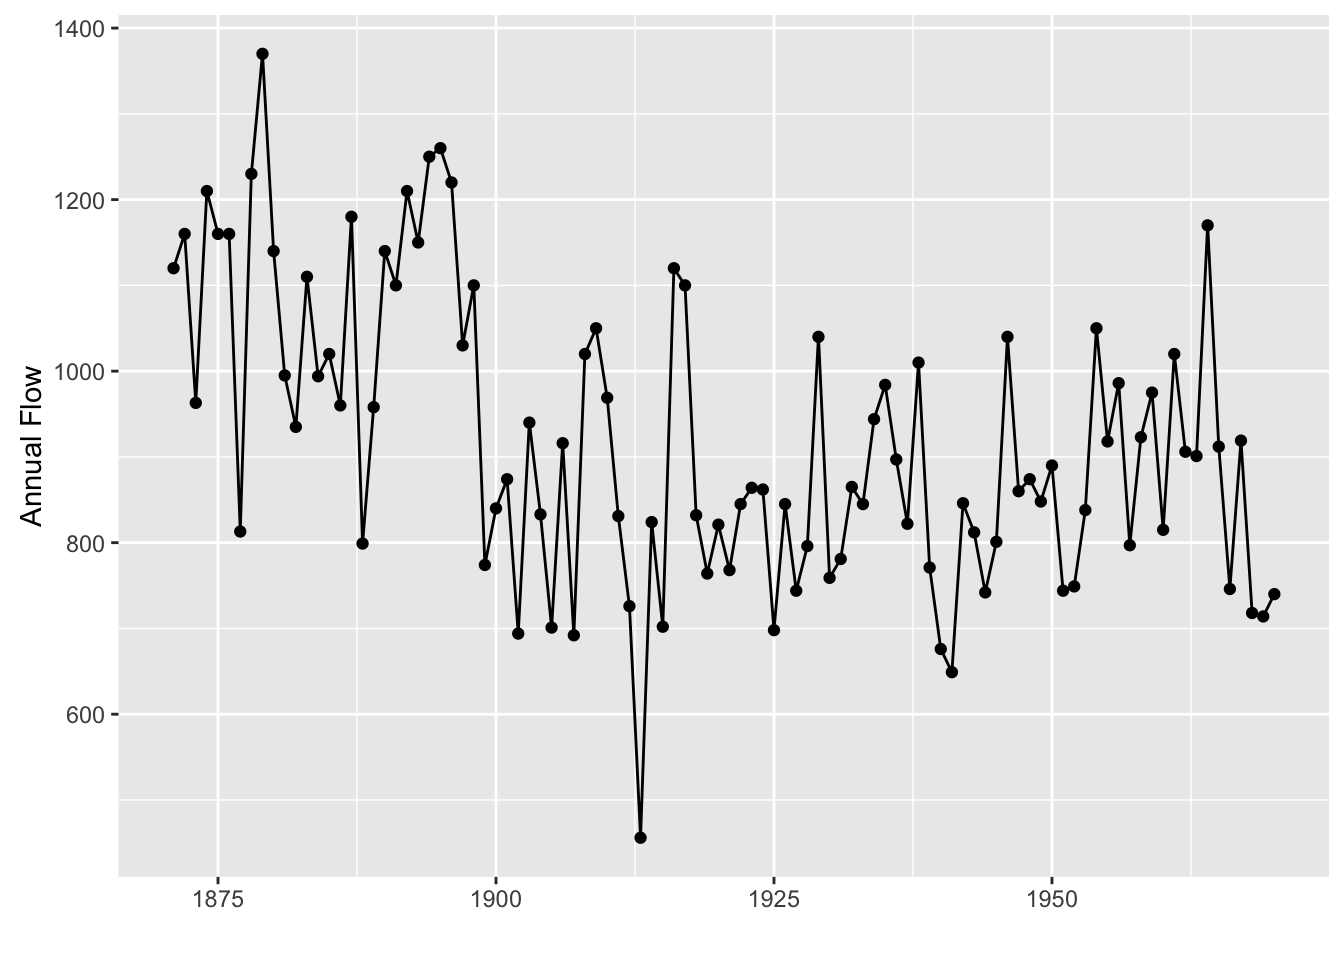
\includegraphics{example-Nile_files/figure-latex/Nile_plot-1.pdf}

\subsection{Local Level Model}\label{local-level-model}

The Nile data can be modeled as a local level model, \[
\begin{aligned}[t]
y_t &= \mu_t + \varepsilon_t & \varepsilon_t & \sim N(0, \sigma_{\varepsilon}^2) \\
\mu_{t + 1} &= \mu_t + \eta_t &
\eta_t & \sim N(0, \sigma^2_{\eta})
\end{aligned}
\]

\begin{verbatim}
functions {
  #include ssm.stan
}
data {
  int<lower = 1> n;
  vector[1] y[n];
  vector<lower = 0.0>[1] a1;
  cov_matrix[1] P1;
  real<lower = 0.0> y_scale;
}
transformed data {
  // system matrices
  matrix[1, 1] T;
  matrix[1, 1] Z;
  matrix[1, 1] R;
  vector[1] c;
  vector[1] d;
  int m;
  int p;
  int q;
  int filter_sz;
  m = 1;
  p = 1;
  q = 1;
  T[1, 1] = 1.0;
  Z[1, 1] = 1.0;
  R[1, 1] = 1.0;
  c[1] = 0.0;
  d[1] = 0.0;
  filter_sz = ssm_filter_size(m, p);
}
parameters {
  real<lower = 0.0> sigma_eta;
  real<lower = 0.0> sigma_epsilon;
}
transformed parameters {
  matrix[1, 1] H;
  matrix[1, 1] Q;
  H[1, 1] = pow(sigma_epsilon, 2);
  Q[1, 1] = pow(sigma_eta * sigma_epsilon, 2);
}
model {
  y ~ ssm_constant_lpdf(d, Z, H, c, T, R, Q, a1, P1);
  sigma_epsilon ~ cauchy(0.0, y_scale);
  sigma_eta ~ cauchy(0.0, 1.0);
}
generated quantities {
  vector[filter_sz] filtered[n];
  vector[1] alpha[n];
  vector[1] eta[n];
  vector[1] eps[n];
  // filtering
  filtered = ssm_filter(y,
    rep_array(d, 1),
    rep_array(Z, 1),
    rep_array(H, 1),
    rep_array(c, 1),
    rep_array(T, 1),
    rep_array(R, 1),
    rep_array(Q, 1), a1, P1);
  // sampling states
  alpha = ssm_simsmo_states_rng(filtered,
    rep_array(d, 1),
    rep_array(Z, 1),
    rep_array(H, 1),
    rep_array(c, 1),
    rep_array(T, 1),
    rep_array(R, 1),
    rep_array(Q, 1), a1, P1);
  eps = ssm_simsmo_eps_rng(filtered,
    rep_array(d, 1),
    rep_array(Z, 1),
    rep_array(H, 1),
    rep_array(c, 1),
    rep_array(T, 1),
    rep_array(R, 1),
    rep_array(Q, 1), a1, P1);
  eta = ssm_simsmo_eta_rng(filtered,
    rep_array(d, 1),
    rep_array(Z, 1),
    rep_array(H, 1),
    rep_array(c, 1),
    rep_array(T, 1),
    rep_array(R, 1),
    rep_array(Q, 1), a1, P1);
}
\end{verbatim}

\begin{Shaded}
\begin{Highlighting}[]
\NormalTok{local_level_mod <-}\StringTok{ }\KeywordTok{ssm_stan_model}\NormalTok{(}\StringTok{"local_level.stan"}\NormalTok{)}
\end{Highlighting}
\end{Shaded}

\begin{Shaded}
\begin{Highlighting}[]
\NormalTok{nile_1_data <-}\StringTok{ }\KeywordTok{within}\NormalTok{(}\KeywordTok{list}\NormalTok{(), \{}
  \NormalTok{y <-}\StringTok{ }\KeywordTok{matrix}\NormalTok{(Nile_$flow)}
  \NormalTok{n <-}\StringTok{ }\KeywordTok{nrow}\NormalTok{(y)}
  \NormalTok{a1 <-}\StringTok{ }\KeywordTok{array}\NormalTok{(}\DecValTok{0}\NormalTok{, }\DecValTok{1}\NormalTok{)}
  \NormalTok{P1 <-}\StringTok{ }\KeywordTok{matrix}\NormalTok{(}\DecValTok{10} \NormalTok{^}\StringTok{ }\DecValTok{7}\NormalTok{)}
  \NormalTok{y_scale <-}\StringTok{ }\KeywordTok{sd}\NormalTok{(Nile_$flow)}
\NormalTok{\})}
\NormalTok{nile_1_samples <-}
\StringTok{  }\KeywordTok{sampling}\NormalTok{(local_level_mod,}
           \DataTypeTok{chains =} \DecValTok{1}\NormalTok{,}
           \DataTypeTok{iter =} \DecValTok{500}\NormalTok{,}
           \DataTypeTok{data =} \NormalTok{nile_1_data)}
\CommentTok{#> }
\CommentTok{#> SAMPLING FOR MODEL 'local_level' NOW (CHAIN 1).}
\CommentTok{#> }
\CommentTok{#> Chain 1, Iteration:   1 / 500 [  0%]  (Warmup)}
\CommentTok{#> Chain 1, Iteration:  50 / 500 [ 10%]  (Warmup)}
\CommentTok{#> Chain 1, Iteration: 100 / 500 [ 20%]  (Warmup)}
\CommentTok{#> Chain 1, Iteration: 150 / 500 [ 30%]  (Warmup)}
\CommentTok{#> Chain 1, Iteration: 200 / 500 [ 40%]  (Warmup)}
\CommentTok{#> Chain 1, Iteration: 250 / 500 [ 50%]  (Warmup)}
\CommentTok{#> Chain 1, Iteration: 251 / 500 [ 50%]  (Sampling)}
\CommentTok{#> Chain 1, Iteration: 300 / 500 [ 60%]  (Sampling)}
\CommentTok{#> Chain 1, Iteration: 350 / 500 [ 70%]  (Sampling)}
\CommentTok{#> Chain 1, Iteration: 400 / 500 [ 80%]  (Sampling)}
\CommentTok{#> Chain 1, Iteration: 450 / 500 [ 90%]  (Sampling)}
\CommentTok{#> Chain 1, Iteration: 500 / 500 [100%]  (Sampling)}
\CommentTok{#>  Elapsed Time: 6.59256 seconds (Warm-up)}
\CommentTok{#>                6.21903 seconds (Sampling)}
\CommentTok{#>                12.8116 seconds (Total)}
\end{Highlighting}
\end{Shaded}

Now, summarize the MCMC samples using the \texttt{summary} function on
the \texttt{stanfit} object. Additionally, I use the
\texttt{tidy\_stan\_summary} function to make the results of
\texttt{summary} easier to work with. This converts the results of
\texttt{summary} from a list of matrices to a list of data frames, and
also parses the parameter names so that it is easier to select
particular parameter values by name. I also will only use only the
summary statistics for the combined chains.

\begin{Shaded}
\begin{Highlighting}[]
\NormalTok{nile_1_summary <-}\StringTok{ }\KeywordTok{tidy_stan_summary}\NormalTok{(}\KeywordTok{summary}\NormalTok{(nile_1_samples))[[}\StringTok{"all"}\NormalTok{]] %>%}
\StringTok{  }\KeywordTok{left_join}\NormalTok{(Nile_, }\DataTypeTok{by =} \KeywordTok{c}\NormalTok{(}\StringTok{"dim_1"} \NormalTok{=}\StringTok{ "obs"}\NormalTok{))}
\end{Highlighting}
\end{Shaded}

The estimated variances of the observation and state variances,

\begin{Shaded}
\begin{Highlighting}[]
\KeywordTok{filter}\NormalTok{(nile_1_summary, parameter %in%}\StringTok{ }\KeywordTok{c}\NormalTok{(}\StringTok{"H"}\NormalTok{, }\StringTok{"Q"}\NormalTok{)) %>%}
\StringTok{  }\KeywordTok{select}\NormalTok{(parname, mean, se_mean, p2}\FloatTok{.5}\NormalTok{, p97}\FloatTok{.5}\NormalTok{, n_eff, Rhat)}
\CommentTok{#> # A tibble: 2 × 7}
\CommentTok{#>   parname  mean se_mean  p2.5 p97.5 n_eff  Rhat}
\CommentTok{#>     <chr> <dbl>   <dbl> <dbl> <dbl> <dbl> <dbl>}
\CommentTok{#> 1  H[1,1] 15031     301  9607 20772  79.3  1.02}
\CommentTok{#> 2  Q[1,1]  2025     130   433  4996 103.6  1.01}
\end{Highlighting}
\end{Shaded}

are similar to the MLE estimates producted by \texttt{StructTS},

\begin{Shaded}
\begin{Highlighting}[]
\KeywordTok{StructTS}\NormalTok{(Nile_$flow, }\DataTypeTok{type =} \StringTok{"level"}\NormalTok{)}
\CommentTok{#> }
\CommentTok{#> Call:}
\CommentTok{#> StructTS(x = Nile_$flow, type = "level")}
\CommentTok{#> }
\CommentTok{#> Variances:}
\CommentTok{#>   level  epsilon  }
\CommentTok{#>    1469    15099}
\end{Highlighting}
\end{Shaded}

However, since the Bayesian estimates are means, the MLE estimates are
modes, and the posterior distribution of the variances are right skewed,
the means are larger than the posterior modes.

\begin{Shaded}
\begin{Highlighting}[]
\NormalTok{str_keep <-}\StringTok{ }\NormalTok{function(string, pattern) \{}
  \NormalTok{string[}\KeywordTok{str_detect}\NormalTok{(string, pattern)]}
\NormalTok{\}}

\KeywordTok{ggplot}\NormalTok{(}\KeywordTok{filter}\NormalTok{(nile_1_summary, parameter ==}\StringTok{ "alpha"}\NormalTok{),}
       \KeywordTok{aes}\NormalTok{(}\DataTypeTok{x =} \NormalTok{year,}
           \DataTypeTok{ymin =} \NormalTok{mean -}\StringTok{ }\DecValTok{2} \NormalTok{*}\StringTok{ }\NormalTok{sd,}
           \DataTypeTok{ymax =} \NormalTok{mean +}\StringTok{ }\DecValTok{2} \NormalTok{*}\StringTok{ }\NormalTok{sd)) +}
\StringTok{  }\KeywordTok{geom_ribbon}\NormalTok{(}\DataTypeTok{alpha =} \FloatTok{0.3}\NormalTok{) +}
\StringTok{  }\KeywordTok{geom_line}\NormalTok{(}\KeywordTok{aes}\NormalTok{(}\DataTypeTok{y =} \NormalTok{mean)) +}
\StringTok{  }\KeywordTok{geom_point}\NormalTok{(}\KeywordTok{aes}\NormalTok{(}\DataTypeTok{y =} \NormalTok{flow)) +}
\StringTok{  }\KeywordTok{ylab}\NormalTok{(}\StringTok{"Annual river flow"}\NormalTok{) +}
\StringTok{  }\KeywordTok{xlab}\NormalTok{(}\StringTok{"Observation"}\NormalTok{) +}
\StringTok{  }\KeywordTok{theme_minimal}\NormalTok{()}
\end{Highlighting}
\end{Shaded}

\includegraphics{example-Nile_files/figure-latex/nile_1_states-1.pdf}

\textbf{TODO} Diagnostics. What are the relevant Bayesian analogs?

\subsection{Local level with known intervention
(intercept)}\label{local-level-with-known-intervention-intercept}

\begin{Shaded}
\begin{Highlighting}[]
\NormalTok{nile_2_mod <-}\StringTok{ }\KeywordTok{ssm_stan_model}\NormalTok{(}\StringTok{"local_level_reg.stan"}\NormalTok{)}
\end{Highlighting}
\end{Shaded}

\begin{Shaded}
\begin{Highlighting}[]
\NormalTok{nile_2_data <-}\StringTok{ }\NormalTok{nile_1_data}
\NormalTok{nile_2_data[[}\StringTok{"x"}\NormalTok{]] <-}\StringTok{ }\KeywordTok{matrix}\NormalTok{(}\KeywordTok{as.integer}\NormalTok{(Nile_$year >}\StringTok{ }\DecValTok{1899}\NormalTok{))}
\NormalTok{nile_2_data[[}\StringTok{"k"}\NormalTok{]] <-}\StringTok{ }\KeywordTok{ncol}\NormalTok{(nile_2_data[[}\StringTok{"x"}\NormalTok{]])}
\NormalTok{nile_2_samples <-}\StringTok{ }\KeywordTok{sampling}\NormalTok{(nile_2_mod, }\DataTypeTok{chains =} \DecValTok{1}\NormalTok{, }\DataTypeTok{iter =} \DecValTok{500}\NormalTok{,}
                           \DataTypeTok{data =} \NormalTok{nile_2_data)}
\CommentTok{#> }
\CommentTok{#> SAMPLING FOR MODEL 'local_level_reg' NOW (CHAIN 1).}
\CommentTok{#> }
\CommentTok{#> Chain 1, Iteration:   1 / 500 [  0%]  (Warmup)}
\CommentTok{#> Chain 1, Iteration:  50 / 500 [ 10%]  (Warmup)}
\CommentTok{#> Chain 1, Iteration: 100 / 500 [ 20%]  (Warmup)}
\CommentTok{#> Chain 1, Iteration: 150 / 500 [ 30%]  (Warmup)}
\CommentTok{#> Chain 1, Iteration: 200 / 500 [ 40%]  (Warmup)}
\CommentTok{#> Chain 1, Iteration: 250 / 500 [ 50%]  (Warmup)}
\CommentTok{#> Chain 1, Iteration: 251 / 500 [ 50%]  (Sampling)}
\CommentTok{#> Chain 1, Iteration: 300 / 500 [ 60%]  (Sampling)}
\CommentTok{#> Chain 1, Iteration: 350 / 500 [ 70%]  (Sampling)}
\CommentTok{#> Chain 1, Iteration: 400 / 500 [ 80%]  (Sampling)}
\CommentTok{#> Chain 1, Iteration: 450 / 500 [ 90%]  (Sampling)}
\CommentTok{#> Chain 1, Iteration: 500 / 500 [100%]  (Sampling)}
\CommentTok{#>  Elapsed Time: 28.6218 seconds (Warm-up)}
\CommentTok{#>                4.59517 seconds (Sampling)}
\CommentTok{#>                33.2169 seconds (Total)}
\CommentTok{#> The following numerical problems occured the indicated number of times after warmup on chain 1}
\CommentTok{#>                                                                                                      count}
\CommentTok{#> Exception thrown at line 2525: Exception thrown at line 1071: Exception thrown at line 279: multiply    14}
\CommentTok{#> When a numerical problem occurs, the Hamiltonian proposal gets rejected.}
\CommentTok{#> See http://mc-stan.org/misc/warnings.html#exception-hamiltonian-proposal-rejected}
\CommentTok{#> If the number in the 'count' column is small, do not ask about this message on stan-users.}
\end{Highlighting}
\end{Shaded}

\begin{Shaded}
\begin{Highlighting}[]
\NormalTok{nile_2_summary <-}\StringTok{ }\KeywordTok{tidy_stan_summary}\NormalTok{(}\KeywordTok{summary}\NormalTok{(nile_2_samples))[[}\StringTok{"all"}\NormalTok{]] %>%}
\StringTok{  }\KeywordTok{left_join}\NormalTok{(Nile_, }\DataTypeTok{by =} \KeywordTok{c}\NormalTok{(}\StringTok{"dim_1"} \NormalTok{=}\StringTok{ "obs"}\NormalTok{))}
\end{Highlighting}
\end{Shaded}

\begin{Shaded}
\begin{Highlighting}[]
\KeywordTok{ggplot}\NormalTok{(}\KeywordTok{filter}\NormalTok{(nile_2_summary, parameter ==}\StringTok{ "mu"}\NormalTok{),}
       \KeywordTok{aes}\NormalTok{(}\DataTypeTok{x =} \NormalTok{year,}
           \DataTypeTok{ymin =} \NormalTok{mean -}\StringTok{ }\DecValTok{2} \NormalTok{*}\StringTok{ }\NormalTok{sd,}
           \DataTypeTok{ymax =} \NormalTok{mean +}\StringTok{ }\DecValTok{2} \NormalTok{*}\StringTok{ }\NormalTok{sd)) +}
\StringTok{  }\KeywordTok{geom_ribbon}\NormalTok{(}\DataTypeTok{alpha =} \FloatTok{0.3}\NormalTok{) +}
\StringTok{  }\KeywordTok{geom_line}\NormalTok{(}\KeywordTok{aes}\NormalTok{(}\DataTypeTok{y =} \NormalTok{mean)) +}
\StringTok{  }\KeywordTok{geom_point}\NormalTok{(}\KeywordTok{aes}\NormalTok{(}\DataTypeTok{y =} \NormalTok{flow)) +}
\StringTok{  }\KeywordTok{ylab}\NormalTok{(}\StringTok{"Annual river flow"}\NormalTok{) +}
\StringTok{  }\KeywordTok{xlab}\NormalTok{(}\StringTok{"Observation"}\NormalTok{) +}
\StringTok{  }\KeywordTok{theme_minimal}\NormalTok{()}
\end{Highlighting}
\end{Shaded}

\includegraphics{example-Nile_files/figure-latex/nile_2_states-1.pdf}

\subsection{Local Level with known intervention
(variance)}\label{local-level-with-known-intervention-variance}

\begin{Shaded}
\begin{Highlighting}[]
\NormalTok{nile_3_mod <-}\StringTok{ }\KeywordTok{ssm_stan_model}\NormalTok{(}\StringTok{"local_level_interven.stan"}\NormalTok{)}
\end{Highlighting}
\end{Shaded}

\begin{Shaded}
\begin{Highlighting}[]
\NormalTok{nile_3_data <-}\StringTok{ }\NormalTok{nile_1_data}
\NormalTok{nile_3_data[[}\StringTok{"s"}\NormalTok{]] <-}\StringTok{ }\KeywordTok{ifelse}\NormalTok{(Nile_$year ==}\StringTok{ }\DecValTok{1899}\NormalTok{, }\DecValTok{10}\NormalTok{, }\DecValTok{1}\NormalTok{)}
\NormalTok{nile_3_samples <-}\StringTok{ }\KeywordTok{sampling}\NormalTok{(nile_3_mod, }\DataTypeTok{chains =} \DecValTok{1}\NormalTok{, }\DataTypeTok{iter =} \DecValTok{500}\NormalTok{,}
                           \DataTypeTok{data =} \NormalTok{nile_3_data)}
\CommentTok{#> }
\CommentTok{#> SAMPLING FOR MODEL 'local_level_interven' NOW (CHAIN 1).}
\CommentTok{#> }
\CommentTok{#> Chain 1, Iteration:   1 / 500 [  0%]  (Warmup)}
\CommentTok{#> Chain 1, Iteration:  50 / 500 [ 10%]  (Warmup)}
\CommentTok{#> Chain 1, Iteration: 100 / 500 [ 20%]  (Warmup)}
\CommentTok{#> Chain 1, Iteration: 150 / 500 [ 30%]  (Warmup)}
\CommentTok{#> Chain 1, Iteration: 200 / 500 [ 40%]  (Warmup)}
\CommentTok{#> Chain 1, Iteration: 250 / 500 [ 50%]  (Warmup)}
\CommentTok{#> Chain 1, Iteration: 251 / 500 [ 50%]  (Sampling)}
\CommentTok{#> Chain 1, Iteration: 300 / 500 [ 60%]  (Sampling)}
\CommentTok{#> Chain 1, Iteration: 350 / 500 [ 70%]  (Sampling)}
\CommentTok{#> Chain 1, Iteration: 400 / 500 [ 80%]  (Sampling)}
\CommentTok{#> Chain 1, Iteration: 450 / 500 [ 90%]  (Sampling)}
\CommentTok{#> Chain 1, Iteration: 500 / 500 [100%]  (Sampling)}
\CommentTok{#>  Elapsed Time: 5.30866 seconds (Warm-up)}
\CommentTok{#>                4.17269 seconds (Sampling)}
\CommentTok{#>                9.48135 seconds (Total)}
\CommentTok{#> The following numerical problems occured the indicated number of times after warmup on chain 1}
\CommentTok{#>                                                                                                      count}
\CommentTok{#> Exception thrown at line 2523: Exception thrown at line 1071: Exception thrown at line 279: multiply    14}
\CommentTok{#> When a numerical problem occurs, the Hamiltonian proposal gets rejected.}
\CommentTok{#> See http://mc-stan.org/misc/warnings.html#exception-hamiltonian-proposal-rejected}
\CommentTok{#> If the number in the 'count' column is small, do not ask about this message on stan-users.}
\end{Highlighting}
\end{Shaded}

\begin{Shaded}
\begin{Highlighting}[]
\NormalTok{nile_3_summary <-}\StringTok{ }\KeywordTok{tidy_stan_summary}\NormalTok{(}\KeywordTok{summary}\NormalTok{(nile_3_samples))[[}\StringTok{"all"}\NormalTok{]] %>%}
\StringTok{  }\KeywordTok{left_join}\NormalTok{(Nile_, }\DataTypeTok{by =} \KeywordTok{c}\NormalTok{(}\StringTok{"dim_1"} \NormalTok{=}\StringTok{ "obs"}\NormalTok{))}
\end{Highlighting}
\end{Shaded}

\begin{Shaded}
\begin{Highlighting}[]
\KeywordTok{ggplot}\NormalTok{(}\KeywordTok{filter}\NormalTok{(nile_3_summary, parameter ==}\StringTok{ "alpha"}\NormalTok{),}
       \KeywordTok{aes}\NormalTok{(}\DataTypeTok{x =} \NormalTok{year,}
           \DataTypeTok{ymin =} \NormalTok{mean -}\StringTok{ }\DecValTok{2} \NormalTok{*}\StringTok{ }\NormalTok{sd,}
           \DataTypeTok{ymax =} \NormalTok{mean +}\StringTok{ }\DecValTok{2} \NormalTok{*}\StringTok{ }\NormalTok{sd)) +}
\StringTok{  }\KeywordTok{geom_ribbon}\NormalTok{(}\DataTypeTok{alpha =} \FloatTok{0.3}\NormalTok{) +}
\StringTok{  }\KeywordTok{geom_line}\NormalTok{(}\KeywordTok{aes}\NormalTok{(}\DataTypeTok{y =} \NormalTok{mean)) +}
\StringTok{  }\KeywordTok{geom_point}\NormalTok{(}\KeywordTok{aes}\NormalTok{(}\DataTypeTok{y =} \NormalTok{flow)) +}
\StringTok{  }\KeywordTok{ylab}\NormalTok{(}\StringTok{"Annual river flow"}\NormalTok{) +}
\StringTok{  }\KeywordTok{xlab}\NormalTok{(}\StringTok{"Observation"}\NormalTok{) +}
\StringTok{  }\KeywordTok{theme_minimal}\NormalTok{()}
\end{Highlighting}
\end{Shaded}

\includegraphics{example-Nile_files/figure-latex/nile_3_states-1.pdf}

\subsection{Local Level model with Sparse State
Disturbances}\label{local-level-model-with-sparse-state-disturbances}

\begin{Shaded}
\begin{Highlighting}[]
\NormalTok{nile_4_mod <-}\StringTok{ }\KeywordTok{ssm_stan_model}\NormalTok{(}\StringTok{"local_level_tvvar.stan"}\NormalTok{)}
\end{Highlighting}
\end{Shaded}

\begin{Shaded}
\begin{Highlighting}[]
\NormalTok{nile_4_data <-}\StringTok{ }\NormalTok{nile_1_data}
\NormalTok{nile_4_data[[}\StringTok{"s"}\NormalTok{]] <-}\StringTok{ }\DecValTok{1} \NormalTok{/}\StringTok{ }\KeywordTok{nrow}\NormalTok{(Nile_)}
\NormalTok{nile_4_samples <-}\StringTok{ }\KeywordTok{sampling}\NormalTok{(nile_4_mod, }\DataTypeTok{chains =} \DecValTok{1}\NormalTok{, }\DataTypeTok{iter =} \DecValTok{500}\NormalTok{,}
                           \DataTypeTok{data =} \NormalTok{nile_4_data)}
\CommentTok{#> }
\CommentTok{#> SAMPLING FOR MODEL 'local_level_tvvar' NOW (CHAIN 1).}
\CommentTok{#> }
\CommentTok{#> Chain 1, Iteration:   1 / 500 [  0%]  (Warmup)}
\CommentTok{#> Chain 1, Iteration:  50 / 500 [ 10%]  (Warmup)}
\CommentTok{#> Chain 1, Iteration: 100 / 500 [ 20%]  (Warmup)}
\CommentTok{#> Chain 1, Iteration: 150 / 500 [ 30%]  (Warmup)}
\CommentTok{#> Chain 1, Iteration: 200 / 500 [ 40%]  (Warmup)}
\CommentTok{#> Chain 1, Iteration: 250 / 500 [ 50%]  (Warmup)}
\CommentTok{#> Chain 1, Iteration: 251 / 500 [ 50%]  (Sampling)}
\CommentTok{#> Chain 1, Iteration: 300 / 500 [ 60%]  (Sampling)}
\CommentTok{#> Chain 1, Iteration: 350 / 500 [ 70%]  (Sampling)}
\CommentTok{#> Chain 1, Iteration: 400 / 500 [ 80%]  (Sampling)}
\CommentTok{#> Chain 1, Iteration: 450 / 500 [ 90%]  (Sampling)}
\CommentTok{#> Chain 1, Iteration: 500 / 500 [100%]  (Sampling)}
\CommentTok{#>  Elapsed Time: 30.9826 seconds (Warm-up)}
\CommentTok{#>                11.9361 seconds (Sampling)}
\CommentTok{#>                42.9187 seconds (Total)}
\CommentTok{#> The following numerical problems occured the indicated number of times after warmup on chain 1}
\CommentTok{#>                                                                                                      count}
\CommentTok{#> Exception thrown at line 2524: Exception thrown at line 1071: Exception thrown at line 279: multiply    11}
\CommentTok{#> When a numerical problem occurs, the Hamiltonian proposal gets rejected.}
\CommentTok{#> See http://mc-stan.org/misc/warnings.html#exception-hamiltonian-proposal-rejected}
\CommentTok{#> If the number in the 'count' column is small, do not ask about this message on stan-users.}
\end{Highlighting}
\end{Shaded}

\begin{Shaded}
\begin{Highlighting}[]
\NormalTok{nile_4_summary <-}\StringTok{ }\KeywordTok{tidy_stan_summary}\NormalTok{(}\KeywordTok{summary}\NormalTok{(nile_4_samples))[[}\StringTok{"all"}\NormalTok{]] %>%}
\StringTok{  }\KeywordTok{left_join}\NormalTok{(Nile_, }\DataTypeTok{by =} \KeywordTok{c}\NormalTok{(}\StringTok{"dim_1"} \NormalTok{=}\StringTok{ "obs"}\NormalTok{))}
\end{Highlighting}
\end{Shaded}

\begin{Shaded}
\begin{Highlighting}[]
\KeywordTok{ggplot}\NormalTok{(}\KeywordTok{filter}\NormalTok{(nile_4_summary, parameter ==}\StringTok{ "alpha"}\NormalTok{),}
       \KeywordTok{aes}\NormalTok{(}\DataTypeTok{x =} \NormalTok{year,}
           \DataTypeTok{ymin =} \NormalTok{mean -}\StringTok{ }\DecValTok{2} \NormalTok{*}\StringTok{ }\NormalTok{sd,}
           \DataTypeTok{ymax =} \NormalTok{mean +}\StringTok{ }\DecValTok{2} \NormalTok{*}\StringTok{ }\NormalTok{sd)) +}
\StringTok{  }\KeywordTok{geom_ribbon}\NormalTok{(}\DataTypeTok{alpha =} \FloatTok{0.3}\NormalTok{) +}
\StringTok{  }\KeywordTok{geom_line}\NormalTok{(}\KeywordTok{aes}\NormalTok{(}\DataTypeTok{y =} \NormalTok{mean)) +}
\StringTok{  }\KeywordTok{geom_point}\NormalTok{(}\KeywordTok{aes}\NormalTok{(}\DataTypeTok{y =} \NormalTok{flow)) +}
\StringTok{  }\KeywordTok{ylab}\NormalTok{(}\StringTok{"Annual river flow"}\NormalTok{) +}
\StringTok{  }\KeywordTok{xlab}\NormalTok{(}\StringTok{"Observation"}\NormalTok{) +}
\StringTok{  }\KeywordTok{theme_minimal}\NormalTok{()}
\end{Highlighting}
\end{Shaded}

\includegraphics{example-Nile_files/figure-latex/nile_4_states-1.pdf}

\chapter{Stan Functions}\label{stan-functions}

State space functionality for Stan is provided as a set of user-defined
functions.

Add the following line to the Stan model file in which depends on these
functions.

\begin{verbatim}
functions {
  #include ssm.stan
  // other functions ...
}
\end{verbatim}

To actually include the functions in the model, you need to use the
function \texttt{stanc\_builder}, instead of \texttt{stan} or
\texttt{stanc}:

\begin{Shaded}
\begin{Highlighting}[]
\NormalTok{model <-}\StringTok{ }\KeywordTok{stanc_builder}\NormalTok{(}\StringTok{"yourmodel.stan"}\NormalTok{, }\DataTypeTok{isystem =} \StringTok{"path/to/ssm/"}\NormalTok{)}
\KeywordTok{stan}\NormalTok{(}\DataTypeTok{model_code =} \NormalTok{model$model_code)}
\end{Highlighting}
\end{Shaded}

\section{Utility Functions}\label{utility-functions}

\subsection{to\_symmetric\_matrix}\label{to_symmetric_matrix}

\textbf{Arguments}

\begin{itemize}
\tightlist
\item
  \texttt{x}: An \(n \times n\) matrix
\end{itemize}

\textbf{returns} An \(n \times n\) symmetric matrix, \(0.5 (x + x')\).

Ensure a matrix is symmetric

\begin{verbatim}
matrix to_symmetric_matrix(matrix x) {
  return 0.5 * (x + x ');
}

\end{verbatim}

\subsection{to\_matrix\_colwise}\label{to_matrix_colwise}

\textbf{Arguments}

\begin{itemize}
\tightlist
\item
  \texttt{v}: An \(n \times m\) vector.
\item
  \texttt{m}: Number of rows in the vector
\item
  \texttt{n}: Number of columns in the vector
\end{itemize}

\textbf{returns} A \(m \times n\) matrix containting the elements from
\texttt{v}

Convert vector to a matrix (column-major).

\begin{verbatim}
matrix to_matrix_colwise(vector v, int m, int n) {
  matrix[m, n] res;
  int k;
  k = 1;
  // by col
  for (j in 1:n) {
    // by row
    for (i in 1:m) {
      res[i, j] = v[k];
      k = k + 1;
    }
  }
  return res;
}

\end{verbatim}

\subsection{matrix\_pow}\label{matrix_pow}

\textbf{Arguments}

\begin{itemize}
\tightlist
\item
  \texttt{A}: The matrix to take the power of
\item
  \texttt{n}: The order of the power. This is sepcified as a real number
  to avoid compiler warnings, but only the integer part is used.
\end{itemize}

\textbf{returns} None

Calculate the power of a matrix, \(\mat{A}^n\).

\begin{verbatim}
matrix matrix_pow(matrix A, real n);


matrix matrix_pow(matrix A, real n) {
  real nn;
  nn = floor(n);
  if (nn == 0) {
    return diag_matrix(rep_vector(1., rows(A)));
  } else if (nn == 1) {
    return A;
  } else if (nn > 1) {
    # recurively this is n log n.
    if (fmod(nn, 2.) > 0) {
      # If odd
      return A * matrix_pow(A, nn - 1);
    } else {
      # If even
      return matrix_pow(A, nn / 2) * matrix_pow(A, nn / 2);
    }
  } else {
    # n < 0
    reject("Only non-negative values of n are allowed");
    return A;
  }
}

// // This is the definition in the Stan book and uses an int n.
// // It requires n multiplications
//
// matrix matrix_pow(matrix A, int n);
//
// matrix matrix_pow(matrix A, int n) {
//   if (n == 0.) {
//     return diag_matrix(rep_vector(1., rows(A)));
//   } else {
//     return a * matrix_pow(A, n - 1);
//   }


\end{verbatim}

\subsection{symmat\_size}\label{symmat_size}

\textbf{Arguments}

\begin{itemize}
\tightlist
\item
  \texttt{n}: The number of rows and columns in the matrix.
\end{itemize}

\textbf{returns} The number of unique elements

Calculate the number of unique elements in a symmetric matrix

The number of unique elements in an \(m \times m\) matrix is
\((m \times (m + 1)) / 2\).

\begin{verbatim}

int symmat_size(int n) {
  int sz;
  // This is calculated iteratively to avoid the Stan warning for
  // integer division
  sz = 0;
  for (i in 1:n) {
    sz = sz + i;
  }
  return sz;
}

\end{verbatim}

\subsection{find\_symmat\_dim}\label{find_symmat_dim}

\textbf{Arguments}

\begin{itemize}
\tightlist
\item
  \texttt{n}: The number of unique elements in a symmetric matrix.
\end{itemize}

\textbf{returns} The dimension of the associated symmetric matrix.

Given vector with \(n\) elements containing the \(m (m + 1) / 2\)
elements of a symmetric matrix, return \(m\).

\begin{verbatim}
int find_symmat_dim(int n) {
  // This could be solved by finding the positive root of $m = m (m + 1)/2 but
  // Stan doesn't support all the functions necessary to do this.
  int i;
  int remainder;
  remainder = n;
  i = 0;
  while (remainder > 0) {
    i = i + 1;
    remainder = remainder - i;
  }
  return i;
}

\end{verbatim}

\subsection{vector\_to\_symmat}\label{vector_to_symmat}

\textbf{Arguments}

\begin{itemize}
\tightlist
\item
  \texttt{x}: The vector with the unique elements
\item
  \texttt{n}: The dimensions of the returned matrix, \(n \times n\).
\end{itemize}

\textbf{returns} matrix An \(n \times n\) symmetric matrix.

Convert a vector to a symmetric matrix

\begin{verbatim}
matrix vector_to_symmat(vector x, int n) {
  matrix[n, n] m;
  int k;
  k = 1;
  // for column
  for (j in 1:n) {
    // for row
    for (i in j:n) {
      m[i, j] = x[k];
      if (i != j) {
        m[j, i] = m[i, j];
      }
      k = k + 1;
    }
  }
  return m;
}

\end{verbatim}

\subsection{symmat\_to\_vector}\label{symmat_to_vector}

\textbf{Arguments}

\begin{itemize}
\tightlist
\item
  \texttt{x}: An \(n \times n\) matrix.
\end{itemize}

\textbf{returns} A \(n (n + 1) / 2\) vector with the unique elements in
\(x\).

Convert an \(n \times n\) symmetric matrix to a length \(n (n + 1) / 2\)
vector containing its unique elements.

\begin{verbatim}

vector symmat_to_vector(matrix x) {
  vector[symmat_size(min(rows(x), cols(x)))] v;
  int m;
  int k;
  k = 1;
  m = min(rows(x), cols(x));
  // if x is m x n symmetric, then this will return
  // only parts of an m x m matrix.
  for (j in 1:m) {
    for (i in j:m) {
      v[k] = x[i, j];
      k = k + 1;
    }
  }
  return v;
}

\end{verbatim}

\subsection{rep\_lower\_triangular\_matrix}\label{rep_lower_triangular_matrix}

\textbf{Arguments}

\begin{itemize}
\tightlist
\item
  \texttt{x}: Value used for the non-zero elements of the matrix.
\item
  \texttt{m}: number of rows
\item
  \texttt{n}: number of columns
\item
  \texttt{diag}: If true, then include 1's on the diagonal.
\end{itemize}

\textbf{returns} An \(m \times n\) lower triangular matrix

Fill in an lower triangular matrix.

\begin{verbatim}

matrix rep_lower_triangular_matrix(real x, int m, int n, int diag) {
  matrix[m, n] A;
  for (i in 1:m) {
    for (j in 1:n) {
      if (i > j) {
        A[i, j] = x;
      } else if (i == j) {
        if (diag) {
          A[i, j] = x;
        } else {
          A[i, j] = 0.;
        }
      } else {
        A[i, j] = 0.;
      }
    }
  }
  return A;
}

\end{verbatim}

\subsection{rep\_upper\_triangular\_matrix}\label{rep_upper_triangular_matrix}

\textbf{Arguments}

\begin{itemize}
\tightlist
\item
  \texttt{x}: Value used for the non-zero elements of the matrix.
\item
  \texttt{m}: number of rows
\item
  \texttt{n}: number of columns
\item
  \texttt{diag}: If true, then include 1's on the diagonal.
\end{itemize}

\textbf{returns} An \(m \times n\) upper triangular matrix

Fill in an upper triangular matrix

\begin{verbatim}

matrix rep_upper_triangular_matrix(real x, int m, int n, int diag) {
  matrix[m, n] A;
  for (i in 1:m) {
    for (j in 1:n) {
      # if row less than column
      if (i < j) {
        A[i, j] = x;
      } else if (i == j) {
        if (diag) {
          A[i, j] = x;
        } else {
          A[i, j] = 0.;
        }
      } else {
        A[i, j] = 0.;
      }
    }
  }
  return A;
}

\end{verbatim}

\subsection{rep\_diagonal\_matrix}\label{rep_diagonal_matrix}

\textbf{Arguments}

\begin{itemize}
\tightlist
\item
  \texttt{x}: Value used for the non-zero elements of the matrix.
\item
  \texttt{m}: number of rows
\item
  \texttt{n}: number of columns
\item
  \texttt{k}: Index of the diagonal
\end{itemize}

\textbf{returns} An \(m \times n\) upper triangular matrix

Create a diagonal \(m \times n\) matrix with values \(x\) on the
\(k\)-th diagonal.

\begin{verbatim}

matrix rep_diagonal_matrix(real x, int m, int n, int k) {
  matrix[m, n] A;
  int mn;
  A = rep_matrix(0., m, n);
  mn = min(m, n);
  if (k >= 0) {
    for (i in 1:min(m, n - k)) {
      A[i, i + k] = x;
    }
  } else {
    for (i in 1:min(m + k, n)) {
      A[i - k, i] = x;
    }
  }
  return A;
}

\end{verbatim}

\subsection{fill\_matrix}\label{fill_matrix}

\textbf{Arguments}

\begin{itemize}
\tightlist
\item
  \texttt{x}: A \(p \times q\), \(p \leq m\), \(\q \leq n\) matrix
\item
  \texttt{m}: Number of rows in the returned matrix
\item
  \texttt{n}: Number of columns in the returned matrix
\item
  \texttt{i}: Indices mapping the rows of \(A\) to the rows in the
  output matrix
\item
  \texttt{j}: Indices mapping the columns of \(A\) to the columns of the
  output matrix
\item
  \texttt{a}: The default value in the returned matrix
\end{itemize}

\textbf{returns} A \(m \times n\) matrix

Given a \(p \times q\) matrix \(\mat{X}\), default value \(a\), and
indexes \(\vec{I} = i_1, ..., i_p\), and \(\vec{J} = j_1, ...j_q\),
return a \(m \times n\) matrix where \(m \geq p\), \(n \geq q\), where
\[
Y_{k, l} =
\begin{cases}
X_{i, j} & \text{if $k = i$, $l = j$, for some $i \in \vec{I}$, $j \in \vec{J}$,} \\
a & \text{otherwise} .
\end{cases}
\]

\begin{verbatim}

matrix fill_matrix(matrix x, int m, int n, int[] i, int[] j, real a) {
  matrix[m, n] ret;
  ret = rep_matrix(a, m, n);
  ret[i, j] = x;
  return ret;
}

\end{verbatim}

\subsection{fill\_vector}\label{fill_vector}

\textbf{Arguments}

\begin{itemize}
\tightlist
\item
  \texttt{x}: A \(p \times q\), \(p \leq m\), \(\q \leq n\) matrix
\item
  \texttt{n}: Number of elements in the returned vector
\item
  \texttt{i}: Indices mapping the rows of \(A\) to the rows in the
  output matrix
\item
  \texttt{a}: The default value in the returned vector
\end{itemize}

\textbf{returns} A \(n \times 1\) matrix

Given an \(m \times 1\) vector \(\vec{x}\), an integer \(n \geq m\), a
default value \(a\), and indexes \(\vec{I} = i_1, ..., i_m \in 1:n\),
return a \(n \times 1\) vector where y\_\{j\} =

\begin{cases}
x_{i} & \text{if $j = i$ for some $i \in \vec{I}$,} \\
a & \text{otherwise}
\end{cases}

. \$\$

\begin{verbatim}

vector fill_vector(vector x, int n, int[] i, real a) {
  vector[n] ret;
  ret = rep_vector(a, n);
  ret[i] = x;
  return ret;
}

\end{verbatim}

\subsection{int\_sum\_true}\label{int_sum_true}

\textbf{Arguments}

\begin{itemize}
\tightlist
\item
  \texttt{x}: An array of length \(n\) of integers
\end{itemize}

\textbf{returns} An integer between 0 and \(n\).

For an array of integers, return the indexes where it is greater than
zero.

\begin{verbatim}

int int_sum_true(int[] x) {
  int n;
  n = 0;
  for (i in 1:num_elements(x)) {
    if (int_step(x[i])) {
      n = n + 1;
    }
  }
  return n;
}

\end{verbatim}

\subsection{int\_sum\_false}\label{int_sum_false}

\textbf{Arguments}

\begin{itemize}
\tightlist
\item
  \texttt{x}: An array of length \(n\) of integers
\end{itemize}

\textbf{returns} An integer between 0 and \(n\).

For an array of integers, return the indexes where it is less than or
equal to zero.

\begin{verbatim}

int int_sum_false(int[] x) {
  int n;
  n = 0;
  for (i in 1:num_elements(x)) {
    if (! int_step(x[i])) {
      n = n + 1;
    }
  }
  return n;
}


\end{verbatim}

\subsection{mask\_indexes}\label{mask_indexes}

\textbf{Arguments}

\begin{itemize}
\tightlist
\item
  \texttt{x}: An array of length \(n\) of integers
\item
  \texttt{n}: The number of false values in \texttt{x}.
\end{itemize}

\textbf{returns} An array of integers with elements having values
between 1 and \(m\).

For an array of integers, \texttt{x}, return the indexes where mask is
not true (\texttt{x{[}i{]}\ \textless{}=\ 0}). The primary use of this
function is where \texttt{x} represents indicators for missing values,
and it is used to extract the indexes of non-missing values.

\begin{verbatim}

int[] mask_indexes(int[] x, int n) {
  int idx[n];
  int j;
  j = 1;
  if (n > 0) {
    for (i in 1:num_elements(x)) {
      if (! int_step(x[i]) && j <= n) {
        idx[j] = i;
        j = j + 1;
      }
    }
  }
  return idx;
}


\end{verbatim}

\subsection{select\_indexes}\label{select_indexes}

\textbf{Arguments}

\begin{itemize}
\tightlist
\item
  \texttt{x}: An array of length \(m\) of integers
\item
  \texttt{n}: The number of true values in \texttt{x}.
\end{itemize}

\textbf{returns} An array of integers with elements having values
between 1 and \(m\).

For an array of integers, \texttt{x}, return the indexes where the
elements are true (\texttt{x{[}i{]}\ \textgreater{}\ 0}). The primary
use of this function is where \texttt{x} represents indicators for
non-missing values, and it is used to extract the indexes of non-missing
values.

\begin{verbatim}

int[] select_indexes(int[] x, int n) {
  int idx[n];
  int j;
  j = 1;
  if (n > 0) {
    for (i in 1:num_elements(x)) {
      if (int_step(x[i]) && j <= n) {
        idx[j] = i;
        j = j + 1;
      }
    }
  }
  return idx;
}

\end{verbatim}

\subsection{normal2\_rng}\label{normal2_rng}

\textbf{Arguments}

\begin{itemize}
\tightlist
\item
  \texttt{mu}: mean
\item
  \texttt{sigma}: variance
\end{itemize}

\textbf{returns} A value drawn from the specified normal distribution.

Draw samples from a normal distribution with mean \texttt{mu} and scale
\texttt{sigma}. Unlike the built-in \texttt{normal\_rng()}, this allows
for \texttt{sigma\ =\ 0}.

\begin{verbatim}

real normal2_rng(real mu, real sigma) {
  real y;
  if (sigma <= 0) {
    y = mu;
  } else {
    y = normal_rng(mu, sigma);
  }
  return y;
}

\end{verbatim}

\subsection{cholesky\_decompose2}\label{cholesky_decompose2}

\textbf{Arguments}

\begin{itemize}
\tightlist
\item
  \texttt{A}: An \(n \times n\) matrix
\end{itemize}

\textbf{returns} An \(n \times n\) lower-triangular matrix

Calculate the Cholesky decomposition of a matrix. Unlike the built-in
function, this handles cases in which the matrix has 0's on the
diagonal.

\begin{verbatim}

matrix cholesky_decompose2(matrix A) {
  matrix[rows(A), cols(A)] L;
  int n;
  int nonzero[rows(A)];
  int num_nonzero;
  n = rows(A);
  for (i in 1:n) {
    nonzero[i] = (A[i, i] > 0);
  }
  num_nonzero = sum(nonzero);
  if (num_nonzero == n) {
    L = cholesky_decompose(A);
  } else if (num_nonzero == 0) {
    L = rep_matrix(0.0, n, n);
  } else {
    int idx[num_nonzero];
    vector[n] eps;
    idx = select_indexes(nonzero, num_nonzero);
    L = rep_matrix(0.0, n, n);
    L[idx, idx] = cholesky_decompose(A[idx, idx]);
  }
  return L;
}


\end{verbatim}

\subsection{multi\_normal2\_rng}\label{multi_normal2_rng}

\textbf{Arguments}

\begin{itemize}
\tightlist
\item
  \texttt{mu}: An \(n \times 1\) vector of the means
\item
  \texttt{Sigma}: An \(n \times n\) lower triangular matrix with
  covariance matrix.
\end{itemize}

\textbf{returns} An \(n \times 1\) vector drawn from the specified
multivariate normal distribution.

Sample from a multivariate normal distribution. Unlike the built-in
\texttt{multi\_normal\_rng}, this function will still draw samples for
deterministic elements in the vector.

\begin{verbatim}

vector multi_normal2_rng(vector mu, matrix Sigma) {
  vector[num_elements(mu)] y;
  int n;
  int nonzero[num_elements(mu)];
  int num_nonzero;
  n = num_elements(mu);
  for (i in 1:n) {
    nonzero[i] = (Sigma[i, i] > 0);
  }
  num_nonzero = sum(nonzero);
  if (num_nonzero == n) {
    y = multi_normal_rng(mu, Sigma);
  } else if (num_nonzero == 0) {
    y = mu;
  } else {
    int idx[num_nonzero];
    vector[n] eps;
    idx = select_indexes(nonzero, num_nonzero);
    eps = rep_vector(0.0, n);
    eps[idx] = multi_normal_rng(rep_vector(0.0, num_nonzero), Sigma[idx, idx]);
    y = mu + eps;
  }
  return y;
}

\end{verbatim}

\subsection{multi\_normal\_cholesky2\_rng}\label{multi_normal_cholesky2_rng}

\textbf{Arguments}

\begin{itemize}
\tightlist
\item
  \texttt{mu}: An \(n \times 1\) vector of the means
\item
  \texttt{L}: An \(n \times n\) lower triangular matrix with the
  Cholesky decomposition of the covariance matrix.
\end{itemize}

\textbf{returns} An \(n \times 1\) vector drawn from the specified
multivariate normal distribution.

Sample from a multivariate normal distribution, parameterized with the
Cholesky decomposition of the covariance matrix. Unlike the built-in
\texttt{multi\_normal\_cholesky\_rng}, this function will still draw
samples for deterministic elements in the vector.

\begin{verbatim}

vector multi_normal_cholesky2_rng(vector mu, matrix L) {
  vector[num_elements(mu)] y;
  int n;
  int nonzero[num_elements(mu)];
  int num_nonzero;
  n = num_elements(mu);
  for (i in 1:n) {
    nonzero[i] = (L[i, i] > 0);
  }
  num_nonzero = sum(nonzero);
  if (num_nonzero == n) {
    y = multi_normal_cholesky_rng(mu, L);
  } else if (num_nonzero == 0) {
    y = mu;
  } else {
    int idx[num_nonzero];
    vector[n] eps;
    idx = select_indexes(nonzero, num_nonzero);
    eps = rep_vector(0.0, n);
    eps[idx] = multi_normal_cholesky_rng(rep_vector(0.0, num_nonzero),
                                         L[idx, idx]);
    y = mu + eps;
  }
  return y;
}


\end{verbatim}

\section{Filtering}\label{filtering-2}

Functions used in filtering and log-likelihood calculations.

\subsection{ssm\_update\_a}\label{ssm_update_a}

\textbf{Arguments}

\begin{itemize}
\tightlist
\item
  \texttt{a}: An \(m \times 1\) vector with the predicted state,
  \(\vec{a}_t\).
\item
  \texttt{c}: An \(m \times 1\) vector with the system intercept,
  \(\vec{c}_t\)
\item
  \texttt{T}: An \(m \times m\) matrix with the transition matrix,
  \(\mat{T}_t\).
\item
  \texttt{v}: A \(p \times 1\) vector with the forecast error,
  \(\vec{v}_t\).
\item
  \texttt{K}: An \(m \times p\) matrix with the Kalman gain,
  \(\mat{K}_t\).
\end{itemize}

\textbf{returns} A \(m \times 1\) vector with the predicted state at
\(t + 1\), \(\vec{a}_{t + 1}\).

Update the expected value of the predicted state,
\(\vec{a}_{t + 1} = \E(\vec{\alpha}_{t + 1} | \vec{y}_{1:t})\),

The predicted state \(\vec{a}_{t + 1}\) is, \[
\vec{a}_{t + 1} = \mat{T}_t \vec{a}_t + \mat{K}_t \vec{v}_t + \vec{c}_t .
\]

\begin{verbatim}

vector ssm_update_a(vector a, vector c, matrix T, vector v, matrix K) {
  vector[num_elements(a)] a_new;
  a_new = T * a + K * v + c;
  return a_new;
}

\end{verbatim}

\subsection{ssm\_update\_P}\label{ssm_update_p}

\textbf{Arguments}

\begin{itemize}
\tightlist
\item
  \texttt{P}: An \(m \times m\) vector with the variance of the
  predicted state, \(\mat{P}_t\).
\item
  \texttt{Z}: A \(p \times m\) matrix with the design matrix,
  \(\mat{Z}_t\).
\item
  \texttt{T}: An \(m \times m\) matrix with the transition matrix,
  \(\mat{T}_t\).
\item
  \texttt{RQR}: A \(m \times m\) matrix with the system covariance
  matrix, \(\mat{R}_t \mat{Q}_t \mat{R}_t'\).
\item
  \texttt{K}: An \(m \times p\) matrix with the Kalman gain,
  \(\mat{K}_t\).
\end{itemize}

\textbf{returns} An \(m \times m\) matrix with the variance of the
state, \(\vec{P}_{t + 1}\).

Update the variance of the state in \(t + 1\),
\(\mat{P}_{t + 1} = \Var(\alpha_{t + 1} | \vec{y}_{1:t})\),

The predicted state variance \(\mat{P}_{t + 1}\) is, \[
\mat{P}_{t + 1} = \mat{T}_t \mat{P}_t (\mat{T}_t - \mat{K}_t \mat{Z}_t)' + \mat{R}_t \mat{Q}_t \mat{R}_t' .
\]

\begin{verbatim}

matrix ssm_update_P(matrix P, matrix Z, matrix T,
                           matrix RQR, matrix K) {
  matrix[rows(P), cols(P)] P_new;
  P_new = to_symmetric_matrix(T * P * (T - K * Z)' + RQR);
  return P_new;
}

\end{verbatim}

\subsection{ssm\_update\_v}\label{ssm_update_v}

\textbf{Arguments}

\begin{itemize}
\tightlist
\item
  \texttt{y}: A \(p \times 1\) vector of the observations,
  \(\vec{y}_t\).
\item
  \texttt{a}: A \(m \times 1\) vector of the states, \(\vec{a}_t\).
\item
  \texttt{d}: A \(p \times 1\) vector with the observation intercept,
  \(\vec{d}_t\).
\item
  \texttt{Z}: A \(p \times m\) matrix with the design matrix,
  \(\mat{Z}_t\).
\end{itemize}

\textbf{returns} A \(p \times 1\) vector of the forecast errors,
\(\vec{v}_t\).

Update the forcast error,
\(\vec{v}_t = \vec{y}_t - \E(\vec{y}_t | \vec{y_{1:(t - 1)}})\)

The forecast error \(\vec{v}_t\) is \[
\vec{v}_t =\vec{y}_t - \mat{Z}_t \vec{a}_t - \vec{d}_t .
\]

\begin{verbatim}

vector ssm_update_v(vector y, vector a, vector d, matrix Z) {
  vector[num_elements(y)] v;
  v = y - Z * a - d;
  return v;
}

\end{verbatim}

\subsection{ssm\_update\_v\_miss}\label{ssm_update_v_miss}

\textbf{Arguments}

\begin{itemize}
\tightlist
\item
  \texttt{y}: A \(p \times 1\) vector of the observations,
  \(\vec{y}_t\).
\item
  \texttt{a}: A \(m \times 1\) vector of the states, \(\vec{a}_t\).
\item
  \texttt{d}: A \(p \times 1\) vector with the observation intercept,
  \(\vec{d}_t\).
\item
  \texttt{Z}: A \(p \times m\) matrix with the design matrix,
  \(\mat{Z}_t\).
\item
  \texttt{p\_t}: The number of non-missing elements of the observation
  vector \(\vec{y}_t\).
\item
  \texttt{y\_idx}: A length \(p\) array of integers indexes with the
  indexes of thenon-missing values of \(y\). Elements \(1:p_t\) should
  be between \(1\) and \(p\); elements \(p_t:p\) are zero, and are not
  used.
\end{itemize}

\textbf{returns} A \(p \times 1\) vector of the forecast errors,
\(\vec{v}_t\).

Update the forcast error, but unlike \texttt{ssm\_update\_v}, allow for
missing values in \(\vec{y}_t\).

The elements of the forecast error \(\vec{v}_t\) is \[
\vec{v}_t =
\begin{cases}
  y_{j,t} - \vec{Z}_{j,.,t} \vec{a}_t - d_{j,t} & \text{if $y_{j,t} not missing.} \\
  0 & \text{if $y_{j,t}$ is missing.}
\end{cases}
\]

\begin{verbatim}

vector ssm_update_v_miss(vector y, vector a, vector d, matrix Z,
                                int p_t, int[] y_idx) {
  vector[num_elements(y)] v;
  int p;
  p = num_elements(y);
  if (p_t < p) {
    v = rep_vector(0., p);
    if (p_t > 0) {
      int idx[p_t];
      vector[p_t] y_star;
      vector[p_t] d_star;
      matrix[p_t, cols(Z)] Z_star;
      idx = y_idx[1:p_t];
      y_star = y[idx];
      d_star = d[idx];
      Z_star = Z[idx, :];
      v[idx] = ssm_update_v(y_star, a, d_star, Z_star);
    }
  } else {
    v = ssm_update_v(y, a, d, Z);
  }
  return v;
}

\end{verbatim}

\subsection{ssm\_update\_F}\label{ssm_update_f}

\textbf{Arguments}

\begin{itemize}
\tightlist
\item
  \texttt{P}: An \(m \times m\) vector with the variance of the
  predicted state, \(\mat{P}_t\).
\item
  \texttt{Z}: A \(p \times m\) matrix with the design matrix,
  \(\mat{Z}_t\).
\item
  \texttt{H}: A \(p \times p\) matrix with the observation covariance
  matrix, \(\mat{H}_t\).
\end{itemize}

\textbf{returns} A \(p \times p\) vector with \(\mat{F}_t\).

Update the variance of the forcast error,
\(\mat{F}_t = \Var(\vec{y}_t - \E(\vec{y}_t | \vec{y_{1:(t - 1)}}))\)

The variance of the forecast error \(\mat{F}_t\) is \[
\mat{F}_t = \mat{Z}_t \mat{P}_t \mat{Z}_t + \mat{H}_t .
\]

\begin{verbatim}

matrix ssm_update_F(matrix P, matrix Z, matrix H) {
  matrix[rows(H), cols(H)] F;
  F = to_symmetric_matrix(quad_form(P, Z') + H);
  return F;
}

\end{verbatim}

\subsection{ssm\_update\_Finv}\label{ssm_update_finv}

\textbf{Arguments}

\begin{itemize}
\tightlist
\item
  \texttt{P}: An \(m \times m\) vector with the variance of the
  predicted state, \(\mat{P}_t\).
\item
  \texttt{Z}: A \(p \times m\) matrix with the design matrix,
  \(\mat{Z}_t\).
\item
  \texttt{H}: A \(p \times p\) matrix with the observation covariance
  matrix, \(\mat{H}_t\).
\end{itemize}

\textbf{returns} A \(p \times p\) vector with \(\mat{F}^{-1}_t\).

Update the precision of the forcast error,
\(\mat{F}^{-1}_t = \Var(\vec{y}_t - \E(\vec{y}_t | \vec{y_{1:(t - 1)}}))^{-1}\)

This is the inverse of \(\mat{F}_t\).

\begin{verbatim}

matrix ssm_update_Finv(matrix P, matrix Z, matrix H) {
  matrix[rows(H), cols(H)] Finv;
  // if can guarantee that F is spd, then take spd inverse.
  Finv = inverse_spd(to_symmetric_matrix(quad_form(P, Z') + H));
  // Finv = inverse(quad_form(P, Z') + H);
  return Finv;
}

\end{verbatim}

\subsection{ssm\_update\_Finv\_miss}\label{ssm_update_finv_miss}

\textbf{Arguments}

\begin{itemize}
\tightlist
\item
  \texttt{P}: An \(m \times m\) vector with the variance of the
  predicted state, \(\mat{P}_t\).
\item
  \texttt{Z}: A \(p \times m\) matrix with the design matrix,
  \(\mat{Z}_t\).
\item
  \texttt{H}: A \(p \times p\) matrix with the observation covariance
  matrix, \(\mat{H}_t\).
\item
  \texttt{p\_t}: The number of non-missing elements in the observation
  vector, \(\vec{y}_t\).
\item
  \texttt{y\_idx}: A length \(p\) array of integers. The first \(p_t\)
  elments of this array indexes of thenon-missing values of \(y\).
  Elements \(1:p_t\) should be between \(1\) and \(p\); elements
  \(p_t:p\) are zero, and are not used.
\end{itemize}

\textbf{returns} A \(p \times p\) vector with \(\mat{F}^{-1}_t\).

Update the precision of the forcast error. Unlike
\texttt{ssm\_update\_Finv}, this allows for missing values in
\texttt{\textbackslash{}vec\{y\}\_\{t\}}. If \(y_{k,t}\) is missing,
then \(F^{-1}_{i,j,t} = 0\) for any \(i = k\) or \(j = k\), otherwise it
is the same as \(\mat{F}^{-1}\) calculated after removing missing
values.

This is the inverse of \(\mat{F}_t\).

\begin{verbatim}

matrix ssm_update_Finv_miss(matrix P, matrix Z, matrix H,
                                   int p_t, int[] y_idx) {
  matrix[rows(H), cols(H)] Finv;
  int p;
  int m;
  p = rows(H);
  m = cols(Z);
  if (p_t < p) {
    Finv = rep_matrix(0., p, p);
    if (p_t > 0) {
      matrix[p_t, m] Z_star;
      matrix[p_t, p_t] H_star;
      int idx[p_t];
      idx = y_idx[1:p_t];
      Z_star = Z[idx, :];
      H_star = H[idx, idx];
      Finv[idx, idx] = ssm_update_Finv(P, Z_star, H_star);
    }
  } else {
    Finv = ssm_update_Finv(P, Z, H);
  }
  return Finv;
}

\end{verbatim}

\subsection{ssm\_update\_K}\label{ssm_update_k}

\textbf{Arguments}

\begin{itemize}
\tightlist
\item
  \texttt{P}: An \(m \times m\) vector with the variance of the
  predicted state, \(P_t\).
\item
  \texttt{Z}: A \(p \times m\) matrix with the design matrix,
  \(\mat{Z}_t\).
\item
  \texttt{T}: An \(m \times m\) matrix with the transition matrix,
  \(\mat{T}_t\).
\item
  \texttt{Finv}: A \(p \times p\) matrix
\end{itemize}

\textbf{returns} An \(m \times p\) matrix with the Kalman gain,
\(\mat{K}_t\).

Update the Kalman gain, \(\mat{K}_t\).

The Kalman gain is \[
\mat{K}_t = \mat{T}_t \mat{P}_t \mat{Z}_t' \mat{F}^{-1}_t .
\]

\begin{verbatim}

matrix ssm_update_K(matrix P, matrix Z, matrix T, matrix Finv) {
  matrix[cols(Z), rows(Z)] K;
  K = T * P * Z' * Finv;
  return K;
}


\end{verbatim}

\subsection{ssm\_update\_L}\label{ssm_update_l}

\textbf{Arguments}

\begin{itemize}
\tightlist
\item
  \texttt{Z}: A \(p \times m\) matrix with the design matrix,
  \(\mat{Z}_t\)
\item
  \texttt{T}: An \(m \times m\) matrix with the transition matrix,
  \(\mat{T}_t\).
\item
  \texttt{K}: An \(m \times p\) matrix with the Kalman gain,
  \(\mat{K}_t\).
\end{itemize}

\textbf{returns} An \(m \times m\) matrix, \(\mat{L}_t\).

Update \(L_t\)

\[
\mat{L}_t = \mat{T}_t - \mat{K}_t \mat{Z}_t .
\]

\begin{verbatim}

matrix ssm_update_L(matrix Z, matrix T, matrix K) {
  matrix[rows(T), cols(T)] L;
  L = T - K * Z;
  return L;
}


\end{verbatim}

\subsection{ssm\_update\_loglik}\label{ssm_update_loglik}

\textbf{Arguments}

\begin{itemize}
\tightlist
\item
  \texttt{v}: A \(p \times 1\) matrix with the forecast error,
  \(\vec{v}_t\).
\item
  \texttt{Finv}: A \(p \times p\) matrix with variance of the forecast
  error, \(\mat{F}^{-1}_t\).
\end{itemize}

\textbf{returns} The log-likelihood

Calculate the log-likelihood of a single observation in a State-space
model

The log-likehood of a single observation in a state-space model is \[
\ell_t = - \frac{1}{2} p \log(2 \pi) - \frac{1}{2} \left(\log|\mat{F}_t| + \vec{v}_t' \mat{F}^{-1}_t \vec{v}_t  \right)
\]

\begin{verbatim}

real ssm_update_loglik(vector v, matrix Finv) {
  real ll;
  int p;
  p = num_elements(v);
  // det(A^{-1}) = 1 / det(A) -> log det(A^{-1}) = - log det(A)
  ll = (- 0.5 *
        (p * log(2 * pi())
         - log_determinant(Finv)
         + quad_form_sym(Finv, v)
       ));
  return ll;
}

\end{verbatim}

\subsection{ssm\_update\_loglik\_miss}\label{ssm_update_loglik_miss}

\textbf{Arguments}

\begin{itemize}
\tightlist
\item
  \texttt{v}: A \(p \times 1\) matrix with the forecast error,
  \(\vec{v}_t\).
\item
  \texttt{Finv}: A \(p \times p\) matrix with variance of the forecast
  error, \(\mat{F}^{-1}_t\).
\item
  \texttt{p\_t}: The number of non-missing elements in the observation
  vector, \(\vec{y}_t\).
\item
  \texttt{y\_idx}: A length \(p\) array of integers. The first \(p_t\)
  elments of this array indexes of thenon-missing values of \(y\).
  Elements \(1:p_t\) should be between \(1\) and \(p\); elements
  \(p_t:p\) are zero, and are not used.
\end{itemize}

\textbf{returns} A \(p \times p\) vector with \(\mat{F}^{-1}_t\).

Calculate the log-likelihood of a single observation in a State-space
model

Unlike \texttt{ssm\_update\_loglik}, this allows for missing values.

\begin{verbatim}

real ssm_update_loglik_miss(vector v, matrix Finv, int p_t, int[] y_idx) {
  real ll;
  int p;
  p = num_elements(v);
  if (p_t == 0) {
    ll = 0.;
  } else if (p_t == p) {
    ll = ssm_update_loglik(v, Finv);
  } else {
    int idx[p_t];
    matrix[p_t, p_t] Finv_star;
    vector[p_t] v_star;
    idx = y_idx[1:p_t];
    Finv_star = Finv[idx, idx];
    v_star = v[idx];
    ll = ssm_update_loglik(v_star, Finv_star);
  }
  return ll;
}


\end{verbatim}

\section{Filtering}\label{filtering-3}

\subsection{ssm\_filter\_idx}\label{ssm_filter_idx}

\textbf{Arguments}

\begin{itemize}
\tightlist
\item
  \texttt{m}: The number of states
\item
  \texttt{p}: The size of the observation vector \(\vec{y}_t\).
\end{itemize}

\textbf{returns} A \(6 \times 3\) integer array containing the indexes
of the return values of the Kalman filter.

Indexes of the return values of the Kalman filter functions:
\texttt{ssm\_filter}.

\texttt{ssm\_filter\_idx} returns a \(6 \times 3\) integer array with
the (length, start index, stop index) of (\(\ell_t\), \(\vec{v}\),
\(\vec{F}^-1\), \(\mat{K}\), \(\vec{a}\), \(\mat{P}\)).

\begin{longtable}[]{@{}llll@{}}
\toprule
value & length & start & stop\tabularnewline
\midrule
\endhead
\(\ell_t\) & \(1\) & \(1\) & \(1\)\tabularnewline
\(\vec{v}\) & \(p\) & \(2\) & \(1 + p\)\tabularnewline
\(\mat{F}^{-1}\) & \(p (p + 1) / 2\) & \(2 + p\) &
\(1 + p + p (p + 1) / 2\)\tabularnewline
\(\mat{K}\) & \(mp\) & \(2 + p + p (p + 1) / 2\) &
\(1 + p + p (p + 1) / 2 + mp\)\tabularnewline
\(\vec{a}_t\) & \(m\) & \(2 + p + p (p + 1) / 2 + mp\) &
\(1 + p + p (p + 1) / 2 + mp + m\)\tabularnewline
\(\mat{P}^t\) & \(m (m + 1) / 2\) & \(2 + p + p (p + 1) / 2 + mp + m\) &
\(1 + p + p (p + 1) / 2 + mp + m (m + 1) / 2\)\tabularnewline
\bottomrule
\end{longtable}

\begin{verbatim}

int[,] ssm_filter_idx(int m, int p) {
  int sz[6, 3];
  // loglike
  sz[1, 1] = 1;
  // v
  sz[2, 1] = p;
  // Finv
  sz[3, 1] = symmat_size(p);
  // K
  sz[4, 1] = m * p;
  // a
  sz[5, 1] = m;
  // P
  sz[6, 1] = symmat_size(m);
  // Fill in start and stop points
  sz[1, 2] = 1;
  sz[1, 3] = sz[1, 2] + sz[1, 1] - 1;
  for (i in 2:6) {
    sz[i, 2] = sz[i - 1, 3] + 1;
    sz[i, 3] = sz[i, 2] + sz[i, 1] - 1;
  }
  return sz;
}

\end{verbatim}

\subsection{ssm\_filter\_size}\label{ssm_filter_size}

\textbf{Arguments}

\begin{itemize}
\tightlist
\item
  \texttt{m}: The number of states
\item
  \texttt{p}: The size of the observation vector \(\vec{y}_t\).
\end{itemize}

\textbf{returns} The number of elements in the vector.

Number of elements in vector containing filter results

\begin{verbatim}

int ssm_filter_size(int m, int p) {
  int sz;
  int idx[6, 3];
  idx = ssm_filter_idx(m, p);
  sz = idx[6, 3];
  return sz;
}

\end{verbatim}

\subsection{ssm\_filter\_get\_loglik}\label{ssm_filter_get_loglik}

\textbf{Arguments}

\begin{itemize}
\tightlist
\item
  \texttt{x}: A vector with results from \texttt{ssm\_filter}.
\item
  \texttt{m}: The number of states
\item
  \texttt{p}: The size of the observation vector \(\vec{y}_t\).
\end{itemize}

\textbf{returns} The log-likelihood \(\ell_t\)

Get the log-likehood from the results of \texttt{ssm\_filter}.

\begin{verbatim}

real ssm_filter_get_loglik(vector x, int m, int p) {
  real y;
  y = x[1];
  return y;
}

\end{verbatim}

\subsection{ssm\_filter\_get\_v}\label{ssm_filter_get_v}

\textbf{Arguments}

\begin{itemize}
\tightlist
\item
  \texttt{x}: vector with results from \texttt{ssm\_filter}.
\item
  \texttt{m}: The number of states
\item
  \texttt{p}: The size of the observation vector \(\vec{y}_t\).
\end{itemize}

\textbf{returns} A \(p \times 1\) vector with the forecast error,
\(\vec{v}_t\).

Get the forecast error from the results of \texttt{ssm\_filter}.

\begin{verbatim}

vector ssm_filter_get_v(vector x, int m, int p) {
  vector[p] y;
  int idx[6, 3];
  idx = ssm_filter_idx(m, p);
  y = segment(x, idx[2, 2], idx[2, 1]);
  return y;
}

\end{verbatim}

\subsection{ssm\_filter\_get\_Finv}\label{ssm_filter_get_finv}

\textbf{Arguments}

\begin{itemize}
\tightlist
\item
  \texttt{x}: vector with results from \texttt{ssm\_filter}.
\item
  \texttt{m}: The number of states
\item
  \texttt{p}: The size of the observation vector \(\vec{y}_t\).
\end{itemize}

\textbf{returns} A \(p \times p\) matrix with the forecast precision,
\(\mat{F}^{-1}_t\).

Get the forecast precision from the results of \texttt{ssm\_filter}.

\begin{verbatim}

matrix ssm_filter_get_Finv(vector x, int m, int p) {
  matrix[p, p] y;
  int idx[6, 3];
  idx = ssm_filter_idx(m, p);
  y = vector_to_symmat(segment(x, idx[3, 2], idx[3, 1]), p);
  return y;
}

\end{verbatim}

\subsection{ssm\_filter\_get\_K}\label{ssm_filter_get_k}

\textbf{Arguments}

\begin{itemize}
\tightlist
\item
  \texttt{x}: vector with results from \texttt{ssm\_filter}.
\item
  \texttt{m}: The number of states
\item
  \texttt{p}: The size of the observation vector \(\vec{y}_t\).
\end{itemize}

\textbf{returns} A \(m \times p\) matrix with the Kalman gain,
\(\mat{K}_t\).

Get the Kalman gain from the results of \texttt{ssm\_filter}.

\begin{verbatim}

matrix ssm_filter_get_K(vector x, int m, int p) {
  matrix[m, p] y;
  int idx[6, 3];
  idx = ssm_filter_idx(m, p);
  y = to_matrix_colwise(segment(x, idx[4, 2], idx[4, 1]), m, p);
  return y;
}

\end{verbatim}

\subsection{ssm\_filter\_get\_a}\label{ssm_filter_get_a}

\textbf{Arguments}

\begin{itemize}
\tightlist
\item
  \texttt{x}: vector with results from \texttt{ssm\_filter}.
\item
  \texttt{m}: The number of states
\item
  \texttt{p}: The size of the observation vector \(\vec{y}_t\).
\end{itemize}

\textbf{returns} An \(m \times 1\) vector with the expected value of the
predicted state, \(\E(\vec{\alpha}_t | \vec{y}_{1:(t-1)}) = \vec{a}_t\).

Get the expected value of the predicted state from the results of
\texttt{ssm\_filter}.

\begin{verbatim}

vector ssm_filter_get_a(vector x, int m, int p) {
  vector[m] y;
  int idx[6, 3];
  idx = ssm_filter_idx(m, p);
  y = segment(x, idx[5, 2], idx[5, 1]);
  return y;
}

\end{verbatim}

\subsection{ssm\_filter\_get\_P}\label{ssm_filter_get_p}

\textbf{Arguments}

\begin{itemize}
\tightlist
\item
  \texttt{x}: vector with results from \texttt{ssm\_filter}.
\item
  \texttt{m}: The number of states
\item
  \texttt{p}: The size of the observation vector \(\vec{y}_t\).
\end{itemize}

\textbf{returns} An \(m \times m\) matrix with the variance of the
predicted state,
\(\Var(\vec{\alpha}_t | \vec{y}_{1:(t-1)}) = \mat{P}_t\).

Get the variance of the predicted state from the results of
\texttt{ssm\_filter}.

\begin{verbatim}

matrix ssm_filter_get_P(vector x, int m, int p) {
  matrix[m, m] y;
  int idx[6, 3];
  idx = ssm_filter_idx(m, p);
  y = vector_to_symmat(segment(x, idx[6, 2], idx[6, 1]), m);
  return y;
}

\end{verbatim}

\subsection{ssm\_filter}\label{ssm_filter}

\textbf{Arguments}

\begin{itemize}
\tightlist
\item
  \texttt{y}: Observations, \(\vec{y}_t\). An array of size \(n\) of
  \(p \times 1\) vectors.
\item
  \texttt{d}: Observation intercept, \(\vec{d}_t\). An array of
  \(p \times 1\) vectors.
\item
  \texttt{Z}: Design matrix, \(\mat{Z}_t\). An array of \(p \times m\)
  matrices.
\item
  \texttt{H}: Observation covariance matrix, \(\mat{H}_t\). An array of
  \(p \times p\) matrices.
\item
  \texttt{c}: State intercept, \(\vec{c}_t\). An array of \(m \times 1\)
  vectors.
\item
  \texttt{T}: Transition matrix, \(\mat{T}_t\). An array of
  \(m \times m\) matrices.
\item
  \texttt{R}: State covariance selection matrix, \(\mat{R} _t\). An
  array of \(p \times q\) matrices.
\item
  \texttt{Q}: State covariance matrix, \(\mat{Q}_t\). An array of
  \(q \times q\) matrices.
\item
  \texttt{a1}: Expected value of the intial state,
  \(a_1 = \E(\alpha_1)\). An \(m \times 1\) matrix.
\item
  \texttt{P1}: Variance of the initial state, \(P_1 = \Var(\alpha_1)\).
  An \(m \times m\) matrix.
\end{itemize}

\textbf{returns} Array of size \(n\) of
\((1 + p + p (p + 1) / 2 + mp + m + m (m + 1) / 2) \times 1\) vectors in
the format described in \texttt{ssm\_filter\_idx}.

Kalman filter

For \texttt{d}, \texttt{Z}, \texttt{H}, \texttt{c}, \texttt{T},
\texttt{R}, \texttt{Q} the array can have a size of 1, if it is not
time-varying, or a size of \(n\) (for \texttt{d}, \texttt{Z},
\texttt{H}) or \(n - 1\) (for \texttt{c}, \texttt{T}, \texttt{R},
\texttt{Q}) if it is time varying.

\texttt{ssm\_filter} runs a forward filter on the state space model and
calculates,

\begin{itemize}
\tightlist
\item
  log-likelihood for each observation, \(\ell_t\).
\item
  Forecast error,
  \(\vec{v}_t = \vec{y}_t - \E(\vec{y}_t | \vec{y}_{1:(t -1)})\).
\item
  Forecast precision, \(\mat{F}^{-1}_t\).
\item
  Kalman gain, \(\mat{K}_t\).
\item
  Predicted states,
  \(\vec{a}_t = \E(\vec{\alpha}_t | \vec{y}_{1:(t -1)})\).
\item
  Variance of the predicted states,
  \(\mat{P}_t = \Var(\vec{\alpha}_t | \vec{y}_{1:(t -1)})\).
\end{itemize}

The results of Kalman filter for a given are returned as a
\(1 + p + p (p + 1) / 2 + m p + m (m + 1) / 2\) vector for each time
period, where \[
(\ell_t, \vec{v}_t', \VEC(\mat{F}^{-1}_t)', \VEC(\mat{K}_t)', \vec{a}_t', \VEC(\mat{P}_t)' )'.
\]

\begin{verbatim}

vector[] ssm_filter(vector[] y,
                    vector[] d, matrix[] Z, matrix[] H,
                    vector[] c, matrix[] T, matrix[] R, matrix[] Q,
                    vector a1, matrix P1) {

  // returned data
  vector[ssm_filter_size(dims(Z)[3], dims(Z)[2])] res[size(y)];
  int q;
  int n;
  int p;
  int m;

  // sizes
  n = size(y); // number of obs
  m = dims(Z)[3]; // number of states
  p = dims(Z)[2]; // obs size
  q = dims(Q)[2]; // number of state disturbances

  //print("Sizes: n = ", m, ", p = ", n, ", m = ", m, ", q = ", q);
  {
    // system matrices for current iteration
    vector[p] d_t;
    matrix[p, m] Z_t;
    matrix[p, p] H_t;
    vector[m] c_t;
    matrix[m, m] T_t;
    matrix[m, q] R_t;
    matrix[q, q] Q_t;
    matrix[m, m] RQR;
    // result matricees for each iteration
    vector[m] a;
    matrix[m, m] P;
    vector[p] v;
    matrix[p, p] Finv;
    matrix[m, p] K;
    real ll;
    int idx[6, 3];

    idx = ssm_filter_idx(m, p);

    d_t = d[1];
    Z_t = Z[1];
    H_t = H[1];
    c_t = c[1];
    T_t = T[1];
    R_t = R[1];
    Q_t = Q[1];
    RQR = quad_form_sym(Q_t, R_t ');
    a = a1;
    P = P1;
    for (t in 1:n) {
      if (t > 1) {
        if (size(d) > 1) {
          d_t = d[t];
        }
        if (size(Z) > 1) {
          Z_t = Z[t];
        }
        if (size(H) > 1) {
          H_t = H[t];
        }
        if (size(c) > 1) {
          c_t = c[t];
        }
        if (size(T) > 1) {
          T_t = T[t];
        }
        if (size(R) > 1) {
          R_t = R[t];
        }
        if (size(Q) > 1) {
          Q_t = Q[t];
        }
        if (size(R) > 1 || size(Q) > 1) {
          RQR = quad_form_sym(Q_t, R_t ');
        }
      }
      // updating
      v = ssm_update_v(y[t], a, d_t, Z_t);
      Finv = ssm_update_Finv(P, Z_t, H_t);
      K = ssm_update_K(P, Z_t, T_t, Finv);
      ll = ssm_update_loglik(v, Finv);
      // saving
      res[t, 1] = ll;
      res[t, idx[2, 2]:idx[2, 3]] = v;
      res[t, idx[3, 2]:idx[3, 3]] = symmat_to_vector(Finv);
      res[t, idx[4, 2]:idx[4, 3]] = to_vector(K);
      res[t, idx[5, 2]:idx[5, 3]] = a;
      res[t, idx[6, 2]:idx[6, 3]] = symmat_to_vector(P);
      // predict a_{t + 1}, P_{t + 1}
      if (t < n) {
        a = ssm_update_a(a, c_t, T_t, v, K);
        P = ssm_update_P(P, Z_t, T_t, RQR, K);
      }
    }
  }
  return res;
}

\end{verbatim}

\subsection{ssm\_filter\_miss}\label{ssm_filter_miss}

\textbf{Arguments}

\begin{itemize}
\tightlist
\item
  \texttt{y}: Observations, \(\vec{y}_t\). An array of size \(n\) of
  \(p \times 1\) vectors.
\item
  \texttt{d}: Observation intercept, \(\vec{d}_t\). An array of
  \(p \times 1\) vectors.
\item
  \texttt{Z}: Design matrix, \(\mat{Z}_t\). An array of \(p \times m\)
  matrices.
\item
  \texttt{H}: Observation covariance matrix, \(\mat{H}_t\). An array of
  \(p \times p\) matrices.
\item
  \texttt{c}: State intercept, \(\vec{c}_t\). An array of \(m \times 1\)
  vectors.
\item
  \texttt{T}: Transition matrix, \(\mat{T}_t\). An array of
  \(m \times m\) matrices.
\item
  \texttt{R}: State covariance selection matrix, \(\mat{R} _t\). An
  array of \(p \times q\) matrices.
\item
  \texttt{Q}: State covariance matrix, \(\mat{Q}_t\). An array of
  \(q \times q\) matrices.
\item
  \texttt{a1}: Expected value of the intial state,
  \(a_1 = \E(\alpha_1)\). An \(m \times 1\) matrix.
\item
  \texttt{P1}: Variance of the initial state, \(P_1 = \Var(\alpha_1)\).
  An \(m \times m\) matrix.
\item
  \texttt{p\_t}: A length \(n\) array with the number of non-missing
  elements in the observation vector, \(\vec{y}_t\), at each
  \(t \in 1, \dots, n\).
\item
  \texttt{y\_idx}: A length \(n \times p\) array of integers. The first
  \(p_t\) elments of this array indexes of thenon-missing values of
  \(y\). Elements \(1:p_t\) should be between \(1\) and \(p\); elements
  \(p_t:p\) are zero, and are not used.
\end{itemize}

\textbf{returns} A \(p \times p\) vector with \(\mat{F}^{-1}_t\).

The function \texttt{ssm\_filter\_miss} runs a Kalman filter like
\texttt{ssm\_filter}, except that it allows for missing values.

In the Kalman filter with missing values, the observation equation is,
\[
\begin{aligned}[t]
\vec{y}^*_{t} &= \vec{d}^*_{t} + \mat{Z}^*_{t} \vec{\alpha}_t + \vec{\varepsilon}^*_t \\
\vec{\varepsilon}^*_t &\sim N(\vec{0}, \mat{H}^*_t)
\end{aligned}
\] where \(\vec{y}^*_{t} = \mat{W}_t \vec{y}_t\),
\(\vec{d}^*_t = \mat{W}_t \vec{d}_t\),
\(\mat{Z}^*_t = \mat{W}_t \mat{Z}_t\),
\(\mat{H}^*_t = \mat{W}_t \mat{H}_t \mat{W}_t\T\), where \(\mat{W}_t\)
selects the non-missing rows of \(\vec{y}_t\).

If all observations

If \(y_{t,j}\) is missing, then

\begin{itemize}
\tightlist
\item
  \(v_{t,j} = 0\)
\item
  \(F^{-1}_{t,.,j} = \vec{0}_{p}\) and F\^{}\{-1\}\emph{\{t,j,.\} =
  \vec{0}}\{p\}\$ if either \$i
\item
  \(K_{t,.,j} = \vec{0}_{m}\)
\end{itemize}

\begin{verbatim}

vector[] ssm_filter_miss(vector[] y,
                          vector[] d, matrix[] Z, matrix[] H,
                          vector[] c, matrix[] T, matrix[] R, matrix[] Q,
                          vector a1, matrix P1, int[] p_t, int[,] y_idx) {

  // returned data
  vector[ssm_filter_size(dims(Z)[3], dims(Z)[2])] res[size(y)];
  int q;
  int n;
  int p;
  int m;

  // sizes
  n = size(y); // number of obs
  m = dims(Z)[3]; // number of states
  p = dims(Z)[2]; // obs size
  q = dims(Q)[2]; // number of state disturbances

  //print("Sizes: n = ", m, ", p = ", n, ", m = ", m, ", q = ", q);
  {
    // system matrices for current iteration
    vector[p] d_t;
    matrix[p, m] Z_t;
    matrix[p, p] H_t;
    vector[m] c_t;
    matrix[m, m] T_t;
    matrix[m, q] R_t;
    matrix[q, q] Q_t;
    matrix[m, m] RQR;
    // result matricees for each iteration
    vector[m] a;
    matrix[m, m] P;
    vector[p] v;
    matrix[p, p] Finv;
    matrix[m, p] K;
    real ll;
    int idx[6, 3];
    idx = ssm_filter_idx(m, p);
    d_t = d[1];
    Z_t = Z[1];
    H_t = H[1];
    c_t = c[1];
    T_t = T[1];
    R_t = R[1];
    Q_t = Q[1];
    RQR = quad_form_sym(Q_t, R_t ');
    a = a1;
    P = P1;
    for (t in 1:n) {
      if (t > 1) {
        if (size(d) > 1) {
          d_t = d[t];
        }
        if (size(Z) > 1) {
          Z_t = Z[t];
        }
        if (size(H) > 1) {
          H_t = H[t];
        }
        if (size(c) > 1) {
          c_t = c[t];
        }
        if (size(T) > 1) {
          T_t = T[t];
        }
        if (size(R) > 1) {
          R_t = R[t];
        }
        if (size(Q) > 1) {
          Q_t = Q[t];
        }
        if (size(R) > 1 || size(Q) > 1) {
          RQR = quad_form_sym(Q_t, R_t ');
        }
      }
      // updating
      v = ssm_update_v_miss(y[t], a, d_t, Z_t, p_t[t], y_idx[t]);
      Finv = ssm_update_Finv_miss(P, Z_t, H_t, p_t[t], y_idx[t]);
      K = ssm_update_K(P, Z_t, T_t, Finv);
      ll = ssm_update_loglik_miss(v, Finv, p_t[t], y_idx[t]);
      // saving
      res[t, 1] = ll;
      res[t, idx[2, 2]:idx[2, 3]] = v;
      res[t, idx[3, 2]:idx[3, 3]] = symmat_to_vector(Finv);
      res[t, idx[4, 2]:idx[4, 3]] = to_vector(K);
      res[t, idx[5, 2]:idx[5, 3]] = a;
      res[t, idx[6, 2]:idx[6, 3]] = symmat_to_vector(P);
      // predict a_{t + 1}, P_{t + 1}
      if (t < n) {
        a = ssm_update_a(a, c_t, T_t, v, K);
        P = ssm_update_P(P, Z_t, T_t, RQR, K);
      }
    }
  }
  return res;
}

\end{verbatim}

\section{Log-likelihood}\label{log-likelihood}

\subsection{ssm\_lpdf}\label{ssm_lpdf}

\textbf{Arguments}

\begin{itemize}
\tightlist
\item
  \texttt{y}: Observations, \(\vec{y}_t\). An array of size \(n\) of
  \(p \times 1\) vectors.
\item
  \texttt{d}: Observation intercept, \(\vec{d}_t\). An array of
  \(p \times 1\) vectors.
\item
  \texttt{Z}: Design matrix, \(\mat{Z}_t\). An array of \(p \times m\)
  matrices.
\item
  \texttt{H}: Observation covariance matrix, \(\mat{H}_t\). An array of
  \(p \times p\) matrices.
\item
  \texttt{c}: State intercept, \(\vec{c}_t\). An array of \(m \times 1\)
  vectors.
\item
  \texttt{T}: Transition matrix, \(\mat{T}_t\). An array of
  \(m \times m\) matrices.
\item
  \texttt{R}: State covariance selection matrix, \(\mat{R} _t\). An
  array of \(p \times q\) matrices.
\item
  \texttt{Q}: State covariance matrix, \(\mat{Q}_t\). An array of
  \(q \times q\) matrices.
\item
  \texttt{a1}: Expected value of the intial state,
  \(a_1 = \E(\alpha_1)\). An \(m \times 1\) matrix.
\item
  \texttt{P1}: Variance of the initial state, \(P_1 = \Var(\alpha_1)\).
  An \(m \times m\) matrix.
\end{itemize}

\textbf{returns} The log-likelihood,
\(p(\vec{y}_{1:n} | \vec{d}, \mat{Z}, \mat{H}, \vec{c}, \mat{T}, \mat{R}, \mat{Q})\),
marginalized over the latent states.

Log-likelihood of a Linear Gaussian State Space Model

For \texttt{d}, \texttt{Z}, \texttt{H}, \texttt{c}, \texttt{T},
\texttt{R}, \texttt{Q} the array can have a size of 1, if it is not
time-varying, or a size of \(n\) (for \texttt{d}, \texttt{Z},
\texttt{H}) or \(n - 1\) (for \texttt{c}, \texttt{T}, \texttt{R},
\texttt{Q}) if it is time varying.

The log-likelihood of a linear Gaussian state space model is, If the the
system matrices and initial conditions are known, the log likelihood is
\[
\begin{aligned}[t]
\log L(\mat{Y}_n) &= \log p(\vec{y}_1, \dots, \vec{y}_n) = \sum_{t = 1}^n \log p(\vec{y}_t | \mat{Y}_{t - 1}) \\
&= - \frac{np}{2} \log 2 \pi - \frac{1}{2} \sum_{t = 1}^n \left( \log \left| \mat{F}_t \right| + \vec{v}\T \mat{F}_t^{-1} \vec{v}_t \right)
\end{aligned} ,
\] where \(\mat{F}_t\) and \(\mat{V}_t\) come from a forward pass of the
Kalman filter.

\begin{verbatim}

real ssm_lpdf(vector[] y,
              vector[] d, matrix[] Z, matrix[] H,
              vector[] c, matrix[] T, matrix[] R, matrix[] Q,
              vector a1, matrix P1) {
  real ll;
  int n;
  int m;
  int p;
  int q;
  n = size(y); // number of obs
  m = dims(Z)[3];
  p = dims(Z)[2];
  q = dims(Q)[2];
  {
    // system matrices for current iteration
    vector[p] d_t;
    matrix[p, m] Z_t;
    matrix[p, p] H_t;
    vector[m] c_t;
    matrix[m, m] T_t;
    matrix[m, q] R_t;
    matrix[q, q] Q_t;
    matrix[m, m] RQR;
    // result matricees for each iteration
    vector[n] ll_obs;
    vector[m] a;
    matrix[m, m] P;
    vector[p] v;
    matrix[p, p] Finv;
    matrix[m, p] K;

    d_t = d[1];
    Z_t = Z[1];
    H_t = H[1];
    c_t = c[1];
    T_t = T[1];
    R_t = R[1];
    Q_t = Q[1];
    RQR = quad_form_sym(Q_t, R_t ');

    a = a1;
    P = P1;
    for (t in 1:n) {
      if (t > 1) {
        if (size(d) > 1) {
          d_t = d[t];
        }
        if (size(Z) > 1) {
          Z_t = Z[t];
        }
        if (size(H) > 1) {
          H_t = H[t];
        }
        if (t < n) {
          if (size(c) > 1) {
            c_t = c[t];
          }
          if (size(T) > 1) {
            T_t = T[t];
          }
          if (size(R) > 1) {
            R_t = R[t];
          }
          if (size(Q) > 1) {
            Q_t = Q[t];
          }
          if (size(R) > 1 || size(Q) > 1) {
            RQR = quad_form_sym(Q_t, R_t ');
          }
        }
      }
      v = ssm_update_v(y[t], a, d_t, Z_t);
      Finv = ssm_update_Finv(P, Z_t, H_t);
      K = ssm_update_K(P, T_t, Z_t, Finv);
      ll_obs[t] = ssm_update_loglik(v, Finv);
      // don't save a, P for last iteration
      if (t < n) {
        a = ssm_update_a(a, c_t, T_t, v, K);
        P = ssm_update_P(P, Z_t, T_t, RQR, K);
      }
    }
    ll = sum(ll_obs);
  }
  return ll;
}

\end{verbatim}

\subsection{ssm\_miss\_lpdf}\label{ssm_miss_lpdf}

\textbf{Arguments}

\begin{itemize}
\tightlist
\item
  \texttt{y}: Observations, \(\vec{y}_t\). An array of size \(n\) of
  \(p \times 1\) vectors.
\item
  \texttt{d}: Observation intercept, \(\vec{d}_t\). An array of
  \(p \times 1\) vectors.
\item
  \texttt{Z}: Design matrix, \(\mat{Z}_t\). An array of \(p \times m\)
  matrices.
\item
  \texttt{H}: Observation covariance matrix, \(\mat{H}_t\). An array of
  \(p \times p\) matrices.
\item
  \texttt{c}: State intercept, \(\vec{c}_t\). An array of \(m \times 1\)
  vectors.
\item
  \texttt{T}: Transition matrix, \(\mat{T}_t\). An array of
  \(m \times m\) matrices.
\item
  \texttt{R}: State covariance selection matrix, \(\mat{R} _t\). An
  array of \(p \times q\) matrices.
\item
  \texttt{Q}: State covariance matrix, \(\mat{Q}_t\). An array of
  \(q \times q\) matrices.
\item
  \texttt{a1}: Expected value of the intial state,
  \(a_1 = \E(\alpha_1)\). An \(m \times 1\) matrix.
\item
  \texttt{P1}: Variance of the initial state, \(P_1 = \Var(\alpha_1)\).
  An \(m \times m\) matrix.
\item
  \texttt{p\_t}: A length \(n\) array with the number of non-missing
  elements in the observation vector, \(\vec{y}_t\), at each
  \(t \in 1, \dots, n\).
\item
  \texttt{y\_idx}: A length \(n \times p\) array of integers. The first
  \(p_t\) elments of this array indexes of thenon-missing values of
  \(y\). Elements \(1:p_t\) should be between \(1\) and \(p\); elements
  \(p_t:p\) are zero, and are not used.
\end{itemize}

\textbf{returns} The log-likelihood
\(p(\vec{y}_{1:n} | \vec{d}_{1:n}, \mat{Z}_{1:n}, \mat{H}_{1:n}, \vec{c}_{1:n}, \mat{T}_{1:n}, \mat{R}_{1:n}, \mat{Q}_{1:n})\).

\begin{verbatim}
real ssm_miss_lpdf(vector[] y,
                   vector[] d, matrix[] Z, matrix[] H,
                   vector[] c, matrix[] T, matrix[] R, matrix[] Q,
                   vector a1, matrix P1, int[] p_t, int[,] y_idx) {
  real ll;
  int n;
  int m;
  int p;
  int q;
  n = size(y); // number of obs
  m = dims(Z)[3];
  p = dims(Z)[2];
  q = dims(Q)[2];
  {
    // system matrices for current iteration
    vector[p] d_t;
    matrix[p, m] Z_t;
    matrix[p, p] H_t;
    vector[m] c_t;
    matrix[m, m] T_t;
    matrix[m, q] R_t;
    matrix[q, q] Q_t;
    matrix[m, m] RQR;
    // result matricees for each iteration
    vector[n] ll_obs;
    vector[m] a;
    matrix[m, m] P;
    vector[p] v;
    matrix[p, p] Finv;
    matrix[m, p] K;

    d_t = d[1];
    Z_t = Z[1];
    H_t = H[1];
    c_t = c[1];
    T_t = T[1];
    R_t = R[1];
    Q_t = Q[1];
    RQR = quad_form_sym(Q_t, R_t ');

    a = a1;
    P = P1;
    for (t in 1:n) {
      if (t > 1) {
        if (size(d) > 1) {
          d_t = d[t];
        }
        if (size(Z) > 1) {
          Z_t = Z[t];
        }
        if (size(H) > 1) {
          H_t = H[t];
        }
        if (t < n) {
          if (size(c) > 1) {
            c_t = c[t];
          }
          if (size(T) > 1) {
            T_t = T[t];
          }
          if (size(R) > 1) {
            R_t = R[t];
          }
          if (size(Q) > 1) {
            Q_t = Q[t];
          }
          if (size(R) > 1 || size(Q) > 1) {
            RQR = quad_form_sym(Q_t, R_t ');
          }
        }
      }
      v = ssm_update_v_miss(y[t], a, d_t, Z_t, p_t[t], y_idx[t]);
      Finv = ssm_update_Finv_miss(P, Z_t, H_t, p_t[t], y_idx[t]);
      K = ssm_update_K(P, Z_t, T_t, Finv);
      ll_obs[t] = ssm_update_loglik_miss(v, Finv, p_t[t], y_idx[t]);
      // don't save a, P for last iteration
      if (t < n) {
        a = ssm_update_a(a, c_t, T_t, v, K);
        P = ssm_update_P(P, Z_t, T_t, RQR, K);
      }
    }
    ll = sum(ll_obs);
  }
  return ll;
}


\end{verbatim}

\section{Time-Invariant Kalman
Filter}\label{time-invariant-kalman-filter}

\subsection{matrix\_diff}\label{matrix_diff}

\textbf{Arguments}

\begin{itemize}
\tightlist
\item
  \texttt{A}: An \(m \times n\) matrix.
\item
  \texttt{B}: An \(m \times n\) matrix.
\end{itemize}

\textbf{returns} If converged, then 1, else 0.

The difference between \(A\) and \(B\) is calculated as, \[
d(A, B) = \max(A - B) / \max(A)
\]

\begin{verbatim}

real matrix_diff(matrix A, matrix B) {
  real eps;
  real norm_AB;
  real norm_A;
  real a;
  real ab;
  int m;
  int n;
  m = rows(A);
  n = cols(A);
  eps = 0.0;
  norm_A = 0.0;
  norm_AB = 0.0;
  for (i in 1:m) {
    for (j in 1:n) {
      a = fabs(A[i, j]);
      ab = fabs(A[i, j] - B[i, j]);
      if (a > norm_A) {
        norm_A = a;
      }
      if (ab > norm_AB) {
        norm_AB = ab;
      }
    }
  }
  eps = norm_AB / norm_A;
  return eps;
}

\end{verbatim}

\subsection{ssm\_constant\_lpdf}\label{ssm_constant_lpdf}

\textbf{Arguments}

\begin{itemize}
\tightlist
\item
  \texttt{y}: Observations, \(\vec{y}_t\). An array of size \(n\) of
  \(p \times 1\) vectors.
\item
  \texttt{d}: Observation intercept, \(\vec{d}_t\). An array of
  \(p \times 1\) vectors.
\item
  \texttt{Z}: Design matrix, \(\mat{Z}_t\). An array of \(p \times m\)
  matrices.
\item
  \texttt{H}: Observation covariance matrix, \(\mat{H}_t\). An array of
  \(p \times p\) matrices.
\item
  \texttt{c}: State intercept, \(\vec{c}_t\). An array of \(m \times 1\)
  vectors.
\item
  \texttt{T}: Transition matrix, \(\mat{T}_t\). An array of
  \(m \times m\) matrices.
\item
  \texttt{R}: State covariance selection matrix, \(\mat{R} _t\). An
  array of \(p \times q\) matrices.
\item
  \texttt{Q}: State covariance matrix, \(\mat{Q}_t\). An array of
  \(q \times q\) matrices.
\item
  \texttt{a1}: Expected value of the intial state,
  \(a_1 = \E(\alpha_1)\). An \(m \times 1\) matrix.
\item
  \texttt{P1}: Variance of the initial state, \(P_1 = \Var(\alpha_1)\).
  An \(m \times m\) matrix.
\end{itemize}

\textbf{returns} The log-likelihood,
\(p(\vec{y}_{1:n} | \vec{d}, \mat{Z}, \mat{H}, \vec{c}, \mat{T}, \mat{R}, \mat{Q})\),
marginalized over the latent states.

Log-likelihood of a Time-Invariant Linear Gaussian State Space Model

Unlike \texttt{ssm\_filter}, this function requires the system matrices
(\texttt{d}, \texttt{Z}, \texttt{H}, \texttt{c}, \texttt{T}, \texttt{R},
\texttt{Q}) to all be time invariant (constant). When the state space
model is time-invariant, then the Kalman recursion for \(\mat{P}_t\)
converges. This function takes advantage of this feature and stops
updating \(\mat{P}_t\) after it converges to a steady state.

\begin{verbatim}

real ssm_constant_lpdf(vector[] y,
                        vector d, matrix Z, matrix H,
                        vector c, matrix T, matrix R, matrix Q,
                        vector a1, matrix P1) {
  real ll;
  int n;
  int m;
  int p;

  n = size(y); // number of obs
  m = cols(Z);
  p = rows(Z);
  {
    vector[n] ll_obs;
    vector[m] a;
    matrix[m, m] P;
    vector[p] v;
    matrix[p, p] Finv;
    matrix[m, p] K;
    matrix[m, m] RQR;
    // indicator for if the filter has converged
    // This only works for time-invariant state space models
    int converged;
    matrix[m, m] P_old;
    real tol;
    real matdiff;
    converged = 0;
    tol = 1e-7;

    RQR = quad_form_sym(Q, R ');
    a = a1;
    P = P1;
    for (t in 1:n) {
      v = ssm_update_v(y[t], a, d, Z);
      if (converged < 1) {
        Finv = ssm_update_Finv(P, Z, H);
        K = ssm_update_K(P, Z, T, Finv);
      }
      ll_obs[t] = ssm_update_loglik(v, Finv);
      // don't save a, P for last iteration
      if (t < n) {
        a = ssm_update_a(a, c, T, v, K);
        // check for convergence
        // should only check for convergence if there are no missing values
        if (converged < 1) {
          P_old = P;
          P = ssm_update_P(P, Z, T, RQR, K);
          matdiff = matrix_diff(P, P_old);
          if (matdiff < tol) {
            converged = 1;
          }
        }
      }
    }
    ll = sum(ll_obs);
  }
  return ll;
}

\end{verbatim}

\section{Common Smoother Functions}\label{common-smoother-functions}

\subsection{ssm\_smooth\_states\_mean}\label{ssm_smooth_states_mean}

\textbf{Arguments}

\begin{itemize}
\tightlist
\item
  \texttt{filter}: The results of \texttt{ssm\_filter}
\item
  \texttt{Z}: Design matrix, \(\mat{Z}_t\). An array of \(p \times m\)
  matrices.
\item
  \texttt{c}: State intercept, \(\vec{c}_t\). An array of \(m \times 1\)
  vectors.
\item
  \texttt{T}: Transition matrix, \(\mat{T}_t\). An array of
  \(m \times m\) matrices.
\item
  \texttt{R}: State covariance selection matrix, \(\mat{R} _t\). An
  array of \(p \times q\) matrices.
\item
  \texttt{Q}: State covariance matrix, \(\mat{Q}_t\). An array of
  \(q \times q\) matrices.
\end{itemize}

\textbf{returns} An array of size \(n\) of \(m \times 1\) vectors
containing \(\hat{\vec{\alpha}}_t\).

The state smoother calculates
\(\hat{\vec{\alpha}}_t = \E(\vec{\alpha}_t | \vec{y}_{1:n})\). \[
\hat{\vec{\alpha}}_{t + 1} = \mat{T}_t \hat{\vec{\alpha}}_{t} + \mat{R}_t \mat{Q}_t \mat{R}'_t \vec{r}_t ,
\] where \(r_t\) is calcualted from the state disturbance smoother. The
smoother is initialized at \(t = 1\) with
\(\hat{\vec{\alpha}}_t = \vec{a}_1 + \mat{P}_1 \vec{r}_0\).

For \texttt{Z}, \texttt{c}, \texttt{T}, \texttt{R}, \texttt{Q} the array
can have a size of 1, if it is not time-varying, or a size of \(n\) (for
\texttt{Z}) or \(n - 1\) (for \texttt{c}, \texttt{T}, \texttt{R},
\texttt{Q}) if it is time varying.

See \autocite[Sec 4.5.3 (eq 4.69)]{DurbinKoopman2012}

\begin{verbatim}

vector[] ssm_smooth_states_mean(vector[] filter,
                              matrix[] Z,
                              vector[] c, matrix[] T, matrix[] R, matrix[] Q) {
  vector[dims(Z)[3]] alpha[size(filter)];
  int n;
  int m;
  int p;
  int q;
  n = size(filter);
  m = dims(Z)[3];
  p = dims(Z)[2];
  q = dims(Q)[2];
  {
    vector[m] r[n + 1];
    vector[p] u;
    vector[m] a1;
    matrix[m, m] P1;
    // filter matrices
    vector[p] v;
    matrix[m, p] K;
    matrix[p, p] Finv;
    // system matrices
    matrix[p, m] Z_t;
    vector[m] c_t;
    matrix[m, m] T_t;
    matrix[m, q] R_t;
    matrix[q, q] Q_t;
    matrix[m, m] RQR;
    // set time-invariant matrices
    if (size(c) == 1) {
      c_t = c[1];
    }
    if (size(Z) == 1) {
      Z_t = Z[1];
    }
    if (size(T) == 1) {
      T_t = T[1];
    }
    if (size(R) == 1) {
      R_t = R[1];
    }
    if (size(Q) == 1) {
      Q_t = Q[1];
    }
    if (size(Q) == 1 && size(R) == 1) {
      RQR = quad_form_sym(Q[1], R[1]');
    }
    // find smoothed state disturbances
    // Since I don't need to calculate the
    // variances of the smoothed disturbances,
    // I reimplement the state distrurbance smoother here
    // removing extraneous parts.
    // r goes from t = n, ..., 1, 0.
    // r_n
    r[n + 1] = rep_vector(0.0, m);
    for (s in 0:(n - 1)) {
      int t;
      // move backwards in time
      t = n - s;
      // update time varying system matrices
      if (size(Z) > 1) {
        Z_t = Z[t];
      }
      if (size(T) > 1) {
        T_t = T[t];
      }
      // get filter values
      K = ssm_filter_get_K(filter[t], m, p);
      v = ssm_filter_get_v(filter[t], m, p);
      Finv = ssm_filter_get_Finv(filter[t], m, p);
      // u_{t - 1}
      u = Finv * v - K ' * r[t + 1];
      // r_{t - 1}
      r[t] = Z_t ' * u + T_t ' * r[t + 1];
    }
    // calculate smoothed states
    a1 = ssm_filter_get_a(filter[1], m, p);
    P1 = ssm_filter_get_P(filter[1], m, p);
    // r[1] = r_0
    alpha[1] = a1 + P1 * r[1];
    // 1:(n - 1) -> \alpha_{2}:\alpha_{n}
    for (t in 1:(n - 1)) {
      if (size(c) > 1) {
        c_t = c[t];
      }
      if (size(T) > 1) {
        T_t = T[t];
      }
      if (size(Q) > 1) {
        Q_t = Q[t];
      }
      if (size(R) > 1) {
        R_t = R[t];
      }
      if (size(Q) > 1 || size(R) > 1) {
        RQR = quad_form_sym(Q_t, R_t');
      }
      // `r[t + 1]` = $r_{t}$
      // alpha_{t + 1} = c_t + T_t * \alpha_t + R_t Q_t R'_t r_t
      alpha[t + 1] = c_t + T_t * alpha[t] + RQR * r[t + 1];
    }
  }
  return alpha;
}


\end{verbatim}

\section{Simulators and Smoothing
Simulators}\label{simulators-and-smoothing-simulators}

\subsection{ssm\_sim\_idx}\label{ssm_sim_idx}

\textbf{Arguments}

\begin{itemize}
\tightlist
\item
  \texttt{m}: The number of states
\item
  \texttt{p}: The length of the observation vector
\item
  \texttt{q}: The number of state disturbances
\end{itemize}

\textbf{returns} A 4 x 3 array of integers

Indexes of each component of \texttt{ssm\_sim\_rng} results.

The returned array has columns (length, start location, and end
location) for rows: \(\vec{y}_t\), \(\vec{\alpha}_t\),
\(\vec{\varepsilon}_t\), and \(\vec{\eta}_t\) in the results of
\texttt{ssm\_sim\_rng}.

\begin{verbatim}

int[,] ssm_sim_idx(int m, int p, int q) {
  int sz[2, 3];
  // y
  sz[1, 1] = p;
  // a
  sz[2, 1] = m;
  // Fill in start and stop points
  sz[1, 2] = 1;
  sz[1, 3] = sz[1, 2] + sz[1, 1] - 1;
  sz[2, 2] = sz[2 - 1, 3] + 1;
  sz[2, 3] = sz[2, 2] + sz[2, 1] - 1;
  return sz;
}

\end{verbatim}

\subsection{ssm\_sim\_size}\label{ssm_sim_size}

\textbf{Arguments}

\begin{itemize}
\tightlist
\item
  \texttt{m}: The number of states
\item
  \texttt{p}: The length of the observation vector
\item
  \texttt{q}: The number of state disturbances
\end{itemize}

\textbf{returns} The number of elements

The number of elements in vectors returned by \texttt{ssm\_sim\_rng}
results.

\begin{verbatim}

int ssm_sim_size(int m, int p, int q) {
  int sz;
  sz = ssm_sim_idx(m, p, q)[2, 3];
  return sz;
}

\end{verbatim}

\subsection{ssm\_sim\_get\_y}\label{ssm_sim_get_y}

\textbf{Arguments}

\begin{itemize}
\tightlist
\item
  \texttt{x}: vector of results from \texttt{ssm\_sim\_rng}
\item
  \texttt{m}: The number of states
\item
  \texttt{p}: The length of the observation vector
\item
  \texttt{q}: The number of state disturbances
\end{itemize}

\textbf{returns} vector A \(p \times 1\) vector with \(\vec{y}_t\).

Extract \(\vec{y}_t\) from vectors returned by \texttt{ssm\_sim\_rng}.

\begin{verbatim}

vector ssm_sim_get_y(vector x, int m, int p, int q) {
  vector[p] y;
  int idx[2, 3];
  idx = ssm_sim_idx(m, p, q);
  y = x[idx[1, 2]:idx[1, 3]];
  return y;
}

\end{verbatim}

\subsection{ssm\_sim\_get\_a}\label{ssm_sim_get_a}

\textbf{Arguments}

\begin{itemize}
\tightlist
\item
  \texttt{x}: vector of results from \texttt{ssm\_sim\_rng}
\item
  \texttt{m}: The number of states
\item
  \texttt{p}: The length of the observation vector
\item
  \texttt{q}: The number of state disturbances
\end{itemize}

\textbf{returns} A \(m \times 1\) vector with \(\vec{\alpha}_t\).

Extract \(\vec{\alpha}_t\) from vectors returne by
\texttt{ssm\_sim\_rng}.

\begin{verbatim}

vector ssm_sim_get_a(vector x, int m, int p, int q) {
  vector[m] a;
  int idx[2, 3];
  idx = ssm_sim_idx(m, p, q);
  a = x[idx[2, 2]:idx[2, 3]];
  return a;
}


\end{verbatim}

\subsection{ssm\_sim\_rng}\label{ssm_sim_rng}

\textbf{Arguments}

\begin{itemize}
\tightlist
\item
  \texttt{n}: Number of time observations to draw, \(t = 1, \dots, n\).
\item
  \texttt{d}: Observation intercept, \(\vec{d}_t\). An array of
  \(p \times 1\) vectors.
\item
  \texttt{Z}: Design matrix, \(\mat{Z}_t\). An array of \(p \times m\)
  matrices.
\item
  \texttt{H}: Observation covariance matrix, \(\mat{H}_t\). An array of
  \(p \times p\) matrices.
\item
  \texttt{c}: State intercept, \(\vec{c}_t\). An array of \(m \times 1\)
  vectors.
\item
  \texttt{T}: Transition matrix, \(\mat{T}_t\). An array of
  \(m \times m\) matrices.
\item
  \texttt{R}: State covariance selection matrix, \(\mat{R} _t\). An
  array of \(p \times q\) matrices.
\item
  \texttt{Q}: State covariance matrix, \(\mat{Q}_t\). An array of
  \(q \times q\) matrices.
\item
  \texttt{a1}: Expected value of the intial state,
  \(a_1 = \E(\alpha_1)\). An \(m \times 1\) matrix.
\item
  \texttt{P1}: Variance of the initial state, \(P_1 = \Var(\alpha_1)\).
  An \(m \times m\) matrix.
\end{itemize}

\textbf{returns} of size \(n\) of vectors with Draw \(\vec{y}_t\),
\(\vec{\alpha}_t\), \(\vec{\eta}_t\) and \(\vec{\varepsilon}_t\). See
the description.

Simulate from a Linear Gaussian State Space model.

For \texttt{d}, \texttt{Z}, \texttt{H}, \texttt{c}, \texttt{T},
\texttt{R}, \texttt{Q} the array can have a size of 1, if it is not
time-varying, or a size of \(n\) (for \texttt{d}, \texttt{Z},
\texttt{H}) or \(n - 1\) (for \texttt{c}, \texttt{T}, \texttt{R},
\texttt{Q}) if it is time varying.

Draw \(\vec{y}_t\), \(\vec{\alpha}_t\), \(\vec{\eta}_t\) and
\(\vec{\varepsilon}_t\) from the state space model, \[
\begin{aligned}[t]
\vec{y}_t &= \vec{d}_t + \mat{Z}_t \vec{\alpha}_t + \vec{\varepsilon}_t,  &
\vec{\varepsilon}_t & \sim N(0, \mat{H}_t), \\
\vec{\alpha}_{t + 1} &= \vec{c}_t + \mat{T}_t \vec{\alpha}_t + \mat{R}_t \vec{\eta}_t,  &
\vec{\eta}_t & \sim N(0, \mat{Q}_t), \\
&& \vec{\alpha}_1 &\sim N(\vec{a}_1, \mat{P}_1) .
\end{aligned}
\]

The returned vectors are of length \(p + m\), in the format, \[
(\vec{y}_t', \vec{\alpha}_t') .
\] Use the functions \texttt{ssm\_sim\_get\_y},
\texttt{ssm\_sim\_get\_a} to extract values from the vector.

\begin{longtable}[]{@{}llll@{}}
\toprule
element & length & start & end\tabularnewline
\midrule
\endhead
\(y_t\) & \(p\) & \(1\) & \(p\)\tabularnewline
\(\alpha\)\_t & \(m\) & \(p + 1\) & \(p + m\)\tabularnewline
\bottomrule
\end{longtable}

\begin{verbatim}

vector[] ssm_sim_rng(int n,
                    vector[] d, matrix[] Z, matrix[] H,
                    vector[] c, matrix[] T, matrix[] R, matrix[] Q,
                    vector a1, matrix P1) {
  vector[ssm_sim_size(dims(Z)[3], dims(Z)[2], dims(Q)[2])] ret[n];
  int p;
  int m;
  int q;
  m = dims(Z)[3];
  p = dims(Z)[2];
  q = dims(Q)[2];
  {
    // system matrices for current iteration
    vector[p] d_t;
    matrix[p, m] Z_t;
    matrix[p, p] H_t;
    matrix[p, p] HL;
    vector[m] c_t;
    matrix[m, m] T_t;
    matrix[m, q] R_t;
    matrix[q, q] Q_t;
    matrix[q, q] QL;
    // outputs
    vector[p] y;
    vector[p] eps;
    vector[m] a;
    vector[q] eta;
    // constants
    vector[p] zero_p;
    vector[q] zero_q;
    vector[m] zero_m;
    int idx[2, 3];

    d_t = d[1];
    Z_t = Z[1];
    H_t = H[1];
    HL = cholesky_decompose2(H_t);
    c_t = c[1];
    T_t = T[1];
    R_t = R[1];
    Q_t = Q[1];
    QL = cholesky_decompose2(Q_t);

    idx = ssm_sim_idx(m, p, q);
    zero_p = rep_vector(0.0, p);
    zero_q = rep_vector(0.0, q);
    zero_m = rep_vector(0.0, m);
    a = multi_normal2_rng(a1, P1);
    for (t in 1:n) {
      // save alpha
      ret[t, idx[2, 2]:idx[2, 3]] = a;
      // set system matrices
      if (t > 1) {
        if (size(d) > 1) {
          d_t = d[t];
        }
        if (size(Z) > 1) {
          Z_t = Z[t];
        }
        if (size(H) > 1) {
          H_t = H[t];
          HL = cholesky_decompose2(H_t);
        }
      }
      // draw forecast error and observed value
      eps = multi_normal_cholesky2_rng(zero_p, HL);
      y = d_t + Z_t * a + eps;
      // save
      ret[t, idx[1, 2]:idx[1, 3]] = y;
      // calculate eta_{t} and a_{t + 1}
      if (t < n) {
        if (size(c) > 1) {
          c_t = c[t];
        }
        if (size(T) > 1) {
          T_t = T[t];
        }
        if (size(R) > 1) {
          R_t = R[t];
        }
        if (size(Q) > 1) {
          Q_t = Q[t];
          QL = cholesky_decompose2(Q_t);
        }
        eta = multi_normal_cholesky2_rng(zero_q, QL);
        a = c_t + T_t * a + R_t * eta;
      }
    }
  }
  return ret;
}

\end{verbatim}

\section{Simulation Smoothers}\label{simulation-smoothers-1}

\subsection{ssm\_simsmo\_states\_rng}\label{ssm_simsmo_states_rng}

\textbf{Arguments}

\begin{itemize}
\tightlist
\item
  \texttt{filter}: A length \(n\) array with results from
  \texttt{ssm\_filter}.
\item
  \texttt{d}: Observation intercept, \(\vec{d}_t\). An array of
  \(p \times 1\) vectors.
\item
  \texttt{Z}: Design matrix, \(\mat{Z}_t\). An array of \(p \times m\)
  matrices.
\item
  \texttt{H}: Observation covariance matrix, \(\mat{H}_t\). An array of
  \(p \times p\) matrices.
\item
  \texttt{c}: State intercept, \(\vec{c}_t\). An array of \(m \times 1\)
  vectors.
\item
  \texttt{T}: Transition matrix, \(\mat{T}_t\). An array of
  \(m \times m\) matrices.
\item
  \texttt{R}: State covariance selection matrix, \(\mat{R} _t\). An
  array of \(p \times q\) matrices.
\item
  \texttt{Q}: State covariance matrix, \(\mat{Q}_t\). An array of
  \(q \times q\) matrices.
\item
  \texttt{a1}: Expected value of the intial state,
  \(a_1 = \E(\alpha_1)\). An \(m \times 1\) matrix.
\item
  \texttt{P1}: Variance of the initial state, \(P_1 = \Var(\alpha_1)\).
  An \(m \times m\) matrix.
\end{itemize}

\textbf{returns} Array of size \(n\) of \(m \times 1\) vectors
containing a single draw from \((\vec{\alpha}_{1:n} | \vec{y}_{1:n})\).

State simulation smoother

Draw samples from the posterior distribution of the states,
\(\tilde{\vec{\alpha}}_{1:n} \sim p(\vec{\alpha}_{1:n} | \vec{y}_{1:n})\).

For \texttt{d}, \texttt{Z}, \texttt{H}, \texttt{c}, \texttt{T},
\texttt{R}, \texttt{Q} the array can have a size of 1, if it is not
time-varying, or a size of \(n\) (for \texttt{d}, \texttt{Z},
\texttt{H}) or \(n - 1\) (for \texttt{c}, \texttt{T}, \texttt{R},
\texttt{Q}) if it is time varying.

This draws samples using mean-correction simulation smoother of
\autocite{DurbinKoopman2002}. See \autocite[Sec 4.9]{DurbinKoopman2012}.

\begin{verbatim}

vector[] ssm_simsmo_states_rng(vector[] filter,
                               vector[] d, matrix[] Z, matrix[] H,
                               vector[] c, matrix[] T, matrix[] R, matrix[] Q,
                               vector a1, matrix P1) {
    vector[dims(Z)[3]] draws[size(filter)];
    int n;
    int p;
    int m;
    int q;
    n = size(filter);
    m = dims(Z)[3];
    p = dims(Z)[2];
    q = dims(Q)[2];
    {
      vector[ssm_filter_size(m, p)] filter_plus[n];
      vector[ssm_sim_size(m, p, q)] sims[n];
      vector[p] y[n];
      vector[m] alpha_hat_plus[n];
      vector[m] alpha_hat[n];
      // Smooth states
      alpha_hat = ssm_smooth_states_mean(filter, Z, c, T, R, Q);
      // simulate unconditional disturbances and observations
      sims = ssm_sim_rng(n, d, Z, H, c, T, R, Q, a1, P1);
      for (i in 1:n) {
        y[i] = ssm_sim_get_y(sims[i], m, p, q);
      }
      // filter with simulated y's
      filter_plus = ssm_filter(y, d, Z, H, c, T, R, Q, a1, P1);
      // mean correct epsilon samples
      alpha_hat_plus = ssm_smooth_states_mean(filter_plus, Z, c, T, R, Q);
      for (i in 1:n) {
        draws[i] = (ssm_sim_get_a(sims[i], m, p, q)
                    - alpha_hat_plus[i]
                    + alpha_hat[i]);
      }
    }
    return draws;
}


\end{verbatim}

\subsection{ssm\_simsmo\_states\_miss\_rng}\label{ssm_simsmo_states_miss_rng}

\textbf{Arguments}

\begin{itemize}
\tightlist
\item
  \texttt{filter}: A length \(n\) array with results from
  \texttt{ssm\_filter}.
\item
  \texttt{d}: Observation intercept, \(\vec{d}_t\). An array of
  \(p \times 1\) vectors.
\item
  \texttt{Z}: Design matrix, \(\mat{Z}_t\). An array of \(p \times m\)
  matrices.
\item
  \texttt{H}: Observation covariance matrix, \(\mat{H}_t\). An array of
  \(p \times p\) matrices.
\item
  \texttt{c}: State intercept, \(\vec{c}_t\). An array of \(m \times 1\)
  vectors.
\item
  \texttt{T}: Transition matrix, \(\mat{T}_t\). An array of
  \(m \times m\) matrices.
\item
  \texttt{R}: State covariance selection matrix, \(\mat{R} _t\). An
  array of \(p \times q\) matrices.
\item
  \texttt{Q}: State covariance matrix, \(\mat{Q}_t\). An array of
  \(q \times q\) matrices.
\item
  \texttt{a1}: Expected value of the intial state,
  \(a_1 = \E(\alpha_1)\). An \(m \times 1\) matrix.
\item
  \texttt{P1}: Variance of the initial state, \(P_1 = \Var(\alpha_1)\).
  An \(m \times m\) matrix.
\item
  \texttt{p\_t}: A length \(n\) array with the number of non-missing
  elements in the observation vector, \(\vec{y}_t\), at each
  \(t \in 1, \dots, n\).
\item
  \texttt{y\_idx}: A length \(n \times p\) array of integers. The first
  \(p_t\) elments of this array indexes of thenon-missing values of
  \(y\). Elements \(1:p_t\) should be between \(1\) and \(p\); elements
  \(p_t:p\) are zero, and are not used.
\end{itemize}

\textbf{returns} Array of size \(n\) of \(m \times 1\) vectors
containing a single draw from \((\vec{\alpha}_{1:n} | \vec{y}_{1:n})\).

State simulation smoother, as in \texttt{ssm\_simsmo\_states\_rng},
allowing for missing values.

\begin{verbatim}

vector[] ssm_simsmo_states_miss_rng(vector[] filter,
                                    vector[] d, matrix[] Z, matrix[] H,
                                    vector[] c, matrix[] T,
                                    matrix[] R, matrix[] Q,
                                    vector a1, matrix P1,
                                    int[] p_t, int[,] y_idx) {
    vector[dims(Z)[3]] draws[size(filter)];
    int n;
    int p;
    int m;
    int q;
    n = size(filter);
    m = dims(Z)[3];
    p = dims(Z)[2];
    q = dims(Q)[2];
    {
      vector[ssm_filter_size(m, p)] filter_plus[n];
      vector[ssm_sim_size(m, p, q)] sims[n];
      vector[p] y[n];
      vector[m] alpha_hat_plus[n];
      vector[m] alpha_hat[n];
      // Smooth states
      alpha_hat = ssm_smooth_states_mean(filter, Z, c, T, R, Q);
      // simulate unconditional disturbances and observations
      sims = ssm_sim_rng(n, d, Z, H, c, T, R, Q, a1, P1);
      for (i in 1:n) {
        y[i] = ssm_sim_get_y(sims[i], m, p, q);
      }
      // filter with simulated y's
      filter_plus = ssm_filter_miss(y, d, Z, H, c, T, R, Q,
                                    a1, P1, p_t, y_idx);
      // mean correct epsilon samples
      alpha_hat_plus = ssm_smooth_states_mean(filter_plus, Z, c, T, R, Q);
      for (i in 1:n) {
        draws[i] = (ssm_sim_get_a(sims[i], m, p, q)
                    - alpha_hat_plus[i]
                    + alpha_hat[i]);
      }
    }
    return draws;
}


\end{verbatim}

\section{Stationary}\label{stationary}

\subsection{pacf\_to\_acf}\label{pacf_to_acf}

\textbf{Arguments}

\begin{itemize}
\tightlist
\item
  \texttt{x}: A vector of coefficients of a partial autocorrelation
  function
\end{itemize}

\textbf{returns} A vector of coefficients of an Autocorrelation function

Partial Autocorrelations to Autocorrelations

\begin{verbatim}

// from R function partrans in arima.c
// https://github.com/wch/r-source/blob/e5b21d0397c607883ff25cca379687b86933d730/src/library/stats/src/arima.c#L439
vector pacf_to_acf(vector x) {
  vector[num_elements(x)] x_new;
  vector[num_elements(x)] work;
  real a;
  int p;
  p = num_elements(x);
  work = x;
  x_new = x;
  if (p > 1) {
    for (j in 2:p) {
      a = x_new[j];
      for (k in 1:(j - 1)) {
        work[k] = work[k] - a * x_new[j - k];
      }
      for (k in 1:j) {
        x_new[k] = work[k];
      }
    }
  }
  return x_new;
}

\end{verbatim}

\subsection{constrain\_stationary}\label{constrain_stationary}

\textbf{Arguments}

\begin{itemize}
\tightlist
\item
  \texttt{x}: An unconstrained vector in \((-\infty, \infty)\)
\end{itemize}

\textbf{returns} A vector of coefficients for a stationary AR or
inverible MA process.

Constrain vector of coefficients to the stationary and intertible region
for AR or MA functions.

See \textcite{Jones1980a}, \textcite{Jones1987a},
\textcite{Monahan1984a}, \textcite{AnsleyKohn1986a}, and the functions
\texttt{tools.constrain\_stationary\_univariate} and
\texttt{tools.unconstraine\_stationary\_univariate} in
\href{http://www.statsmodels.org/dev/statespace.html\#statespace-tools}{statsmodels.tsa.statespace}.

\begin{enumerate}
\def\labelenumi{\arabic{enumi}.}
\tightlist
\item
  Each \(\alpha_j \in (-\infty, \infty)\) is transformed to a partial
  correlation within \((-1, 1)\), with \(\rho_j = \tanh(\alpha_j)\).
\item
  Then the partial correlations are converted to autocorrelation
  coefficients using the Durbin-Levinson recursions: \[
     \]
\end{enumerate}

The transformation is reversed to take autocorrelation coefficients to
an unconstrained \(R^p\) space.

\begin{enumerate}
\def\labelenumi{\arabic{enumi}.}
\tightlist
\item
  Autocorrelation coefficients are transformed to partial
  autocorrelation coefficients, by running the Durbin-Levinson
  recursions in reverse.
\item
  Transform each partial autocorrelation to go from
  \((-1, 1) \to (-\infty, \infty)\) using,
  \(\alpha_j = \atanh(\rho_j)\).
\end{enumerate}

\begin{verbatim}

vector constrain_stationary(vector x) {
  vector[num_elements(x)] r;
  int n;
  n = num_elements(x);
  // transform (-Inf, Inf) to (-1, 1)
  for (i in 1:n) {
    r[i] = tanh(x[i]);
  }
  // Transform PACF to ACF
  return pacf_to_acf(r);
}



\end{verbatim}

\subsection{acf\_to\_pacf}\label{acf_to_pacf}

\textbf{Arguments}

\begin{itemize}
\tightlist
\item
  \texttt{x}: Coeffcients of an autocorrelation function.
\end{itemize}

\textbf{returns} A vector of coefficients of the corresponding partial
autocorrelation function.

Convert coefficients of an autocorrelation function to partial
autocorrelations.

\begin{verbatim}

// from R function invpartrans in arima.c
// https://github.com/wch/r-source/blob/e5b21d0397c607883ff25cca379687b86933d730/src/library/stats/src/arima.c#L525
vector acf_to_pacf(vector x) {
  vector[num_elements(x)] x_new;
  vector[num_elements(x)] work;
  real a;
  int p;
  p = num_elements(x);
  work = x;
  x_new = x;
  // Run the Durbin-Levinson recursions backwards
  if (p > 1) {
    for(i in 0:(p - 2)) {
      int j;
      j = p - i;
      a = x_new[j];
      for(k in 1:(j - 1)) {
        work[k]  = (x_new[k] + a * x_new[j - k]) / (1 - pow(a, 2));
      }
      for (k in 1:j) {
        x_new[k] = work[k];
      }
    }
  }
  return x_new;
}

\end{verbatim}

\subsection{unconstrain\_stationary}\label{unconstrain_stationary}

\textbf{Arguments}

\begin{itemize}
\tightlist
\item
  \texttt{x}: Coeffcients of an autocorrelation function.
\end{itemize}

\textbf{returns} Coefficients of the corresponding partial
autocorrelation function.

Transform from stationary and invertible space to \((-\infty, \infty)\).

\begin{verbatim}

vector unconstrain_stationary(vector x) {
  matrix[num_elements(x), num_elements(x)] y;
  vector[num_elements(x)] r;
  vector[num_elements(x)] z;
  int n;
  n = num_elements(x);
  // Transform ACF to PACF
  r = acf_to_pacf(x);
  // Transform (-1, 1) to (-Inf, Inf)
  for (i in 1:n) {
    z[i] = atanh(r[i]);
  }
  return z;
}

\end{verbatim}

\subsection{kronecker\_prod}\label{kronecker_prod}

\textbf{Arguments}

\begin{itemize}
\tightlist
\item
  \texttt{A}: An \(m \times n\) matrix
\item
  \texttt{B}: A \(p \times q\) matrix
\end{itemize}

\textbf{returns} An \(mp \times nq\) matrix.

The Kronecker product of a \(\mat{A}\) and \(\mat{B}\) is \[
\mat{A} \otimes \mat{B} =
\begin{bmatrix}
a_{11} \mat{B} \cdots a_{1n} \mat{B} \\
\vdots & \ddots & vdots \\
a_{m1} \mat{B} & \cdots & a_{mn} \mat{B}
\end{bmatrix} .
\]

\begin{verbatim}

matrix kronecker_prod(matrix A, matrix B) {
  matrix[rows(A) * rows(B), cols(A) * cols(B)] C;
  int m;
  int n;
  int p;
  int q;
  m = rows(A);
  n = cols(A);
  p = rows(B);
  q = cols(B);
  for (i in 1:m) {
    for (j in 1:n) {
      int row_start;
      int row_end;
      int col_start;
      int col_end;
      row_start = (i - 1) * p + 1;
      row_end = (i - 1) * p + p;
      col_start = (j - 1) * q + 1;
      col_end = (j - 1) * q + q;
      C[row_start:row_end, col_start:col_end] = A[i, j] * B;
    }
  }
  return C;
}

\end{verbatim}

\subsection{stationary\_cov}\label{stationary_cov}

\textbf{Arguments}

\begin{itemize}
\tightlist
\item
  \texttt{T}: The \(m \times m\) transition matrix
\item
  \texttt{RQR}: The \(m \times m\) system covarariance matrix,
  \(\mat{R} \mat{Q} \mat{R}\T\).
\end{itemize}

\textbf{returns} An \(m \times m\) matrix with the stationary covariance
matrix.

Find the covariance of the stationary distribution of an ARMA model

When a system is stationary, the initial covariance \(P_1\) satistfies,
\[
\mat{P}_1 = \mat{T} \mat{P}_1 \mat{T}\T + \mat{R} \mat{Q} \mat{R}\T
\] This can be solved as, \[
(\mat{T} \otimes \mat{T}) \VEC(\mat{P}_1) = \VEC(\mat{R} \mat{Q} \mat{R}\T)
\] where \(\VEC(P_1)\) and \(\VEC(R R')\) are the stacked columns of
\(\mat{P}_1\) and \(\mat{R} \mat{Q} \mat{R}\T\)

Note that in the special case of ARIMA models, \(\mat{Q} = \sigma^2\),
so this simplifies to, \[
(\mat{T} \otimes \mat{T}) \VEC(\mat{Q}_0) = \VEC(\mat{R} \mat{R}\T),
\] where \(P_1 = \sigma^2 \mat{Q}_0\).

In a stationary distribution, the initial mean \(\vec{a}_1 = \vec{c}\).

See \textcite{DurbinKoopman2012}, Sec 5.6.2.

\begin{verbatim}

matrix stationary_cov(matrix T, matrix RQR) {
  matrix[rows(T), cols(T)] P;
  int m;
  m = rows(T);
  // m = 1 is an easy case, so treat it separately
  // since it doesn't require inverting a matrix
  if (m == 1) {
    P[1, 1] = RQR[1, 1] / (1.0 - pow(T[1, 1], 2));
  } else {
    matrix[rows(T) * rows(T), rows(T) * rows(T)] TT;
    vector[rows(T) * rows(T)] RQR_vec;
    int m2;
    m2 = m * m;
    RQR_vec = to_vector(RQR);
    # I_{m^2} - T \otimes T
    TT = - kronecker_prod(T, T);
    for (i in 1:m2) {
      TT[i, i] = 1.0 + TT[i, i];
    }
    P = to_matrix_colwise(inverse(TT) * RQR_vec, m, m);
  }
  return P;
}
\end{verbatim}

\chapter{Other Software}\label{other-software}

This a brief summary of other available software to estimate state space
models with a focus on R and python.

\section{R packages}\label{r-packages}

\textcite{Tusell2011} reviews R packages for state space models (as of
2011). \textcite{Helske2012} includes an more recent review of R
packages implementing state space models.

\begin{itemize}
\item
  The \textbf{stats} package includes functions for univariate Kalman
  filtering and smoothing (\texttt{KalmanLike}, \texttt{KalmanRun},
  \texttt{KalmanSmooth}, \texttt{KalmanForecast}) which are used by
  \texttt{StructTS} and \texttt{arima}.
\item
  dse
\item
  sspir
\item
  dlm
\item
  KFAS
\item
  dlmodeler - provides a unified interface to multiple packages
\item
  rucm: structural time series
\item
  MARSS - maximum likelihood estimation of a large glass of Guassian
  state space models with an EM-algorithm
\end{itemize}

\section{Other}\label{other}

The \href{https://www.jstatsoft.org/issue/view/v041}{JSS Volume 41}
\autocite{CommandeurKoopmanOoms2011} contains articles on state space
implementations in multiple languages

\begin{itemize}
\tightlist
\item
  STAMP \autocite{Mendelssohn2011a}
\item
  Ox/SsfPack \autocite{Pelagatti2011a}
\item
  R \autocite{PetrisPetrone2011a}
\item
  SsfPack in S+FinMetrics \autocite{Zivot2011a}
\item
  Matlab \autocite{PengAston2011a}
\item
  FORTRAN \autocite{Bell2011a}
\item
  eViews \autocite{Bossche2011a}
\item
  RATS \autocite{Doan2011a}
\item
  Stata \autocite{DrukkerGates2011a}
\item
  gretl \autocite{Lucchetti2011a}
\item
  SAS \autocite{Selukar2011a}
\item
  Ox \autocite{Bos2011a}
\end{itemize}

\subsection{Stata}\label{stata}

Stata's \href{http://www.stata.com/manuals14/ts.pdf}{timeseries}
capabilities includes the command \texttt{ssmodels} to estimate general
state space models, as well as common special cases: \texttt{arima}
(SARIMAX models), \texttt{dfactor} (Dynamic Factor), and \texttt{ucm}
(Unobserved Components Models).

\subsection{Python}\label{python}

The {[}statsmodels{]} module {[}statsmodels.tsa{]} contains functions
and classes for time series analysis including autoregressive (AR),
vector autoregressive (VAR), autoregressive moving avergage models
(ARMA), and functions fo Kalman filtering. Currently the Kalman filter
only handles the special univariate case for ARIMA.

The \textbf{statsmodels} module
\href{http://www.statsmodels.org/dev/statespace.html\#}{statsmodels.tsa.statespace}
contains more general state space code. The examples are very good.

An
\href{http://pages.uoregon.edu/cfulton/posts/state_space_mh.html}{example}
of using \texttt{statsmodels.tsa.statespace} and
\href{http://pymcmc.readthedocs.io/en/latest/}{PyMC} to simulate from
the posterior of a state space model. See
\href{http://pages.uoregon.edu/cfulton/posts/state_space_python.html}{State
Space Modeling in Python}.

\textcite{StricklandBurdettMengersenEtAl2014a} introduce
\href{https://bitbucket.org/christophermarkstrickland/pyssm}{PySSM} to
simulate state space models using PyMCMC (not to be confused with the
more popular PyMC).

\printbibliography


\end{document}
